\chapter{同伦类型论}
\label{cha:basics}

同伦类型论的核心新思想是：类型可以被视为同伦论中的空间，或范畴论中的高维群胚。

\index{classical!homotopy theory|(}
\index{higher category theory|(}
我们先简要回顾同伦论与高维范畴论之间的联系。
在经典同伦论中，一个空间 $X$ 是一个配备了拓扑的点集，
\indexsee{space!topological}{topological space}
\index{topological!space}
而点 $x$ 与 $y$ 之间的一条道路则用一个连续映射 $p : [0,1] \to X$ 表示，其中 $p(0) = x$ 且 $p(1) = y$。
\index{path!topological}
\index{topological!path}
可以把这个函数理解为在每个"时刻"给出 $X$ 中的一个点。
对于许多目的而言，道路的严格相等（即逐点相等的函数）是一个过分精细的概念。
例如，我们可以定义道路的拼接运算（若 $p$ 是从 $x$ 到 $y$ 的道路，$q$ 是从 $y$ 到 $z$ 的道路，则拼接 $p \ct q$ 是从 $x$ 到 $z$ 的道路）和取逆运算（$\opp p$ 是从 $y$ 到 $x$ 的道路）。
然而，这些运算之间有一些自然的等式，对于严格相等而言并不成立：
例如，道路 $p \ct \opp p$（它随着时间从 $0$ 到 $1$，从 $x$ 走到 $y$，再沿原路返回）并不严格等于恒等道路（它始终静止在 $x$ 点）。

解决之道在于引入一种更粗略的道路相等概念，称为\emph{同伦}。
\index{homotopy!topological}
一对连续映射 $f : X_1 \to X_2$ 与 $g : X_1\to X_2$ 之间的一个同伦，是一个连续映射 $H : X_1
\times [0, 1] \to X_2$，满足 $H(x, 0) = f (x)$ 与 $H(x, 1) =
g(x)$。
特别地，对于从 $x$ 到 $y$ 的两条道路 $p$ 和 $q$，同伦是一个连续映射 $H : [0,1] \times [0,1] \rightarrow X$，
使得对所有 $s\in [0,1]$，有 $H(s,0) = p(s)$ 和 $H(s,1) = q(s)$。
在这种情况下，我们还要求对所有 $t\in [0,1]$，有 $H(0,t) = x$ 且 $H(1,t)=y$，
从而对每个 $t$，函数 $H(\blank,t)$ 仍然是一条从 $x$ 到 $y$ 的道路；
这类同伦被称为\emph{保端点的}或\emph{相对于端点的}。
在简单的情形中，我们可以把正方形 $[0,1]\times [0,1]$ 在 $H$ 下的像看作"填满"了 $p$ 与 $q$ 之间的"空间"，
尽管对于一般的 $X$ 来说这并不真正有意义；
更好的理解方式是把 $H$ 看作将 $p$ 连续形变为 $q$ 且不移动端点的过程。
由于 $[0,1]\times [0,1]$ 是 2 维的，我们也将 $H$ 称为\emph{道路之间的 2 维道路}。\index{path!2-}

例如，因为 $p \ct \opp p$ 沿同一条路线走出去又走回来，所以你可以将 $p \ct \opp p$ 连续地缩为恒等道路——例如，它不会被空间中的空洞"钩住"。
同伦是一种等价关系，且拼接、取逆等运算都与它相容。
此外，在某点 $x_0$ 处环路\index{loop}的同伦等价类（两条环路 $p$ 和 $q$ 在存在它们之间的\emph{保基点的}同伦时被视为相等，即如上所述的同伦 $H$ 并额外满足对所有 $t$ 有 $H(0,t) =
H(1,t) = x_0$）构成一个群，称为\emph{基本群}。\index{fundamental!group}
这个群是空间的一个\emph{代数不变量}，可用于探究两个空间是否\emph{同伦等价}
（即存在来回的连续映射，其复合均同伦于恒等映射），因为同伦等价的空间具有同构的基本群。

由于同伦本身是一种 2 维道路，自然就有 3 维的\emph{同伦之间的同伦}\index{path!3-}的概念，
进而还有\emph{同伦之间的同伦之间的同伦}，如此等等。
这个由点、道路、同伦、同伦之间的同伦……构成的无限塔，连同基本群等代数运算，是被称为（弱）\emph{$\infty$-群胚}的代数结构的一个实例。
一个 $\infty$-\emph{群胚}\index{.infinity-groupoid@$\infty$-groupoid}包含一组对象，
然后是对象之间的一组\emph{态射}\indexdef{morphism!in an .infinity-groupoid@in an $\infty$-groupoid}，
接着是\emph{态射之间的态射}，依此类推，并配有某种复杂的代数结构；
第 $k$ 层的态射称为\define{$k$-态射 ($k$-morphism)}\indexdef{k-morphism@$k$-morphism}。
每一层的态射都有单位、复合和逆运算，但这些运算具有所谓的"弱性"：
具体来说，它们满足群胚定律（复合的结合律、单位元是复合的单位、逆元可消去）仅在相差一个下一层态射的意义下成立，而这种弱性会引发进一步的结构。
例如，由于态射复合 $p \ct (q \ct r) = (p \ct q) \ct r$ 的结合律本身就是一个更高维的态射，我们需要额外的运算来关联各种结合性证明：
将 $p \ct
(q \ct (r \ct s))$ 用不同方式重新结合为 $((p \ct q) \ct r) \ct s$，就引出了 Mac Lane（麦克兰恩）的五边形\index{pentagon, Mac Lane}。
弱性还会造成不同层次之间非平凡的相互作用。

每个拓扑空间 $X$ 都有一个\emph{基本 $\infty$-群胚}
\index{.infinity-groupoid@$\infty$-groupoid!fundamental}
\index{fundamental!.infinity-groupoid@$\infty$-groupoid}，
其 $k$-态射就是 $X$ 中的 $k$ 维道路。
$\infty$-群胚的弱性直接对应于这样一个事实：道路仅在同伦意义下构成群，其中 $(k+1)$-道路充当 $k$-道路之间的同伦。
此外，将空间视为 $\infty$-群胚的观点保留了足够多的空间信息以开展同伦论：
基本 $\infty$-群胚的构造与一个 $\infty$-群胚作为空间的几何\index{geometric realization}实现构成伴随\index{adjoint!functor}关系，
且该伴随保持同伦论（这称为\emph{同伦假说/定理}，%
\index{hypothesis!homotopy}%
\index{homotopy!hypothesis}%
因为它是假说还是定理取决于如何定义 $\infty$-群胚）。
例如，你可以容易地定义一个 $\infty$-群胚的基本群；而如果你计算一个空间的基本 $\infty$-群胚的基本群，结果将与该空间基本群的经典定义相符。
正是由于这种对应关系，同伦论与高维范畴论紧密相连。

\index{classical!homotopy theory|)}%
\index{higher category theory|)}%

\mentalpause

现在，在同伦类型论中，每个类型都可以被看作具有 $\infty$-群胚的结构。
回想一下，对于任何类型 $A$ 和任意 $x, y : A$，我们都有一个相等类型 $\id[A]{x}{y}$，也写作 $\idtype[A]{x}{y}$ 或简写为 $x = y$。
从逻辑上讲，我们可以将 $x = y$ 的元素看作 $x$ 与 $y$ 相等的证据，或 $x$ 与 $y$ 的相等证明。
此外，类型论（不同于一阶逻辑等系统）允许我们将 $\id[A]{x}{y}$ 的这类元素本身也视为个体，从而成为进一步命题的主语。
因此，我们可以\emph{迭代}相等类型：可以构造相等证明 $p, q$ 之间的相等证明类型 $\id[{(\id[A]{x}{y})}]{p}{q}$，
以及类型 $\id[{(\id[{(\id[A]{x}{y})}]{p}{q})}]{r}{s}$，如此等等。
这个相等类型塔的结构，精确地对应于空间中的连续道路及其间的（高阶）同伦，或一个 $\infty$-群胚\index{.infinity-groupoid@$\infty$-groupoid}。

因此，我们通常将元素$p : \id[A]{x}{y}$称为从 $x$ 到 $y$ 的一条\define{道路（path）}；
\index{path}
我们称 $x$ 为其\define{起点（start point）}
\indexdef{start point of a path}
\indexdef{path!start point of}，
称 $y$ 为其\define{终点（end point）}。
\indexdef{end point of a path}
\indexdef{path!end point of}
两条起点和终点相同的道路$p,q : \id[A]{x}{y}$被称为\define{平行的（parallel）}，
\indexdef{parallel paths}
\indexdef{path!parallel}此时，元素$r : \id[{(\id[A]{x}{y})}]{p}{q}$可以看作一个同伦，或态射之间的态射；
我们通常将其称为\define{2-道路（2-path）}
\indexdef{path!2-}\indexsee{2-path}{path, 2-}%
或\define{2-维道路（2-dimensional path）}。
\index{dimension!of paths}%
\indexsee{2-dimensional path}{path, 2-}\indexsee{path!2-dimensional}{path, 2-}%
类似地，$\id[{(\id[{(\id[A]{x}{y})}]{p}{q})}]{r}{s}$是两个平行2-维道路之间的\define{3-维道路（3-dimensional path）}
\indexdef{path!3-}\indexsee{3-path}{path, 3-}\indexsee{3-dimensional path}{path, 3-}\indexsee{path!3-dimensional}{path, 3-}%
的类型，依此类推。
如果类型 $A$ 是"集合式的"，例如 \nat，那么这些迭代的相等类型将平淡无奇（参见\cref{sec:basics-sets}）；但在一般情况下，它们可以模拟非平凡的同伦类型。

%% (Obviously, the
%% notation ``$\id[A]{x}{y}$'' has its limitations here.  The style
%% $\idtype[A]{x}{y}$ is only slightly better in iterations:
%% $\idtype[{\idtype[{\idtype[A]{x}{y}}]{p}{q}}]{r}{s}$.)

同伦类型论与经典同伦论的一个重要区别在于，同伦类型论以如下意义提供了一种对空间的\emph{综合（synthetic）}描述。
\index{synthetic mathematics}%
\index{geometry, synthetic}%
\index{Euclid of Alexandria}%
综合几何是Euclid ~\cite{Euclid} 风格的几何学：从一些基本概念（点与直线）、构造（连接任意两点的直线）和公理（所有直角都相等）出发，通过逻辑推导出结论。
这与\emph{解析}几何形成对比，
\index{analytic mathematics}%
在解析几何中，点和直线等概念通过 $\R^n$ 中的笛卡尔坐标具体表示——直线是点的集合——而基本构造和公理由此表示导出。
经典同伦论是解析的（空间和道路由点构成），而同伦类型论是综合的：点、道路以及道路之间的道路是基本的、不可分割的、原始的概念。

此外，同伦类型论的一个令人惊叹之处是，所有基本构造和公理——所有高阶群胚结构——都自动从相等类型的归纳原理中产生。
回顾\cref{sec:identity-types}，该原理是说，如果

\begin{itemize}
\item 对于每个 $x,y:A$ 和每个 $p:\id[A]xy$，我们有一个类型 $D(x,y,p)$，且
\item 对于每个 $a:A$，我们有一个元素$d(a):D(a,a,\refl a)$，
\end{itemize}

那么

\begin{itemize}
\item 对于\emph{任意}两个元素 $x,y:A$ 和 $p:\id[A]xy$，都存在一个元素$\indid{A}(D,d,x,y,p):D(x,y,p)$，使得$\indid{A}(D,d,a,a,\refl a) \jdeq d(a)$。
\end{itemize}

换言之，给定依值函数
\begin{align*}
D & :\prd{x,y:A} (\id{x}{y}) \to \type\\
d & :\prd{a:A} D(a,a,\refl{a})
\end{align*}
存在一个依值函数
\[\indid{A}(D,d):\prd{x,y:A}{p:\id{x}{y}} D(x,y,p)\]
使得对每个 $a:A$ 有
\begin{equation}\label{eq:Jconv}
\indid{A}(D,d,a,a,\refl{a})\jdeq d(a)
\end{equation}。
通常，每次应用这个归纳规则时，我们要么不关心所定义的具体函数，要么立即给它另一个名字。

非正式地说，相等类型的归纳原理是说：如果我们想构造一个依赖于相等类型元素 $p:\id[A]xy$ 的对象（或证明一个陈述），那么只需在 $x$ 和 $y$ 判断相等且 $p$ 是自反元素 $\refl{x}:x=x$（判断相等）的特殊情况下进行构造（或证明）即可。
在非正式表述中，我们可以用"由归纳，只需假设……"这样的短语来表达。
这种"归约到自反性情形"的做法，类似于在自然数上作普通归纳证明时归约到"基础情况"和"归纳步骤"，也类似于在对不相交并或析取作分情形讨论时归约到"左情况"和"右情况"。\index{induction principle!for identity type}%

在关于自然数的归纳证明的语境中，"转换规则"~\eqref{eq:Jconv}可能不那么熟悉，但在与之相关的递归定义概念中，却有一个类似的想法。
如果序列\index{sequence} $(a_n)_{n\in \mathbb{N}}$是通过给定 $a_0$ 并用 $a_n$ 表示 $a_{n+1}$ 来定义的，那么结果序列的第 $0$ 项\emph{确实}就是给定的 $a_0$，并且给定的联系 $a_{n+1}$ 与 $a_n$ 的递推关系对结果序列成立。
这一点可能看起来过于显然，不值一提；但倘若我们将递归定义视为计算序列值的算法\index{algorithm}，那么它恰恰就是执行该算法的过程。
规则~\eqref{eq:Jconv} 与此类似：如果我们通过指定 $p$ 为 $\refl{x}:x=x$ 时的值来为所有 $p:x=y$ 定义对象 $f(p)$，那么我们指定的值事实上就是 $f(\refl{x})$ 的值。

这个归纳原理赋予每个类型以 $\infty$-群胚\index{.infinity-groupoid@$\infty$-groupoid}的结构，并使两个类型之间的每个函数具有相应群胚之间的 $\infty$-函子\index{.infinity-functor@$\infty$-functor}结构。
从数学的观点来看，这很有趣，因为它提供了一种处理 $\infty$-群胚的新方法。
从类型论的观点来看，这同样有趣，因为它揭示了与每个类型和函数相关联的新运算。
在本章剩余的部分里，我们将开始探索这种结构。

\section{类型是高阶群胚}
\label{sec:equality}

\index{type!identity|(}%
\index{path|(}%
\index{.infinity-groupoid@$\infty$-groupoid!structure of a type|(}%
我们现在从归纳原理出发，推导高阶群胚结构的初步内容。
我们从相等性的对称性开始，用拓扑学的语言来说，这意味着"道路可以反转"。

\begin{lem}\label{lem:opp}
  对每个类型 $A$ 以及任意 $x,y:A$，存在一个函数
  \begin{equation*}
    (x= y)\to(y= x)
  \end{equation*}
  记作 $p\mapsto \opp{p}$，使得对每个 $x:A$ 有 $\opp{\refl{x}}\jdeq\refl{x}$。
  我们称 $\opp{p}$ 为 $p$ 的\define{逆（inverse）}。
  \indexdef{path!inverse}%
  \indexdef{inverse!of path}%
  \index{equality!symmetry of}%a
  \index{symmetry!of equality}%
\end{lem}

鉴于这是我们第一次将某个陈述表述为"引理"或"定理"，不妨稍作停顿，思考一下这意味着什么。
回想一下，命题（可被证明的陈述）等同于类型，而引理和定理（已被证明的陈述）则等同于\emph{有实例的}类型。
因此，引理或定理的陈述应被转译为一个类型，如 \cref{sec:pat} 所示，而其证明则被转译为该类型的一个实例。
根据全称量词"对每个"的解释，与 \cref{lem:opp} 对应的类型是
\[ \prd{A:\UU}{x,y:A} (x= y)\to(y= x). \]
\cref{lem:opp} 的证明将在于构造该类型的一个元素，即对某个 $f$ 推导出判断 $f:\prd{A:\UU}{x,y:A} (x= y)\to(y= x)$。
然后，我们引入符号 $\opp{(\blank)}$ 来表示这个元素 $f$，其中参数 $A$、$x$ 和 $y$ 被省略并由上下文推断。
（如 \cref{sec:types-vs-sets} 所述，次要陈述"对每个 $x:A$，有 $\opp{\refl{x}}\jdeq\refl{x}$"应被视为一个独立的判断。）

\begin{proof}[第一次证明]
  假设给定 $A:\UU$，
  并令 $D:\prd{x,y:A}(x= y) \to \type$ 为由 $D(x,y,p)\defeq (y= x)$ 定义的类型族。
  换句话说，$D$ 是一个函数，它为任意 $x,y:A$ 和 $p:x=y$ 指派一个类型，即类型 $y=x$。
  于是我们有一个元素
  \begin{equation*}
    d\defeq \lam{x} \refl{x}:\prd{x:A} D(x,x,\refl{x}).
  \end{equation*}
  因此，相等类型的归纳原理给了我们一个元素
  \narrowequation{ \indid{A}(D,d,x,y,p): (y= x)}
  对每个 $p:(x= y)$。
  现在我们可以定义所需的函数 $\opp{(\blank)}$ 为 $\lam{p} \indid{A}(D,d,x,y,p)$，即令 $\opp{p} \defeq \indid{A}(D,d,x,y,p)$。
  转换规则~\eqref{eq:Jconv} 给出了 $\opp{\refl{x}}\jdeq \refl{x}$，如所需。
\end{proof}

我们以非常形式化的风格写出了这个证明，这在大家对相等类型的归纳规则还不熟悉时或许有所帮助。
若追求更形式化，我们可以说 \cref{lem:opp} 及其证明共同构成了判断
\begin{narrowmultline*}
  \lam{A}{x}{y}{p} \indid{A}((\lam{x}{y}{p} (y=x)), (\lam{x} \refl{x}), x, y, p)
  \narrowbreak : \prd{A:\UU}{x,y:A} (x= y)\to(y= x)
\end{narrowmultline*}
（以及一个额外的相等判断）。
然而，最终我们更倾向于使用更自然的语言，如下面这个等价的证明所示。

\begin{proof}[第二次证明]
  我们想为每对 $x,y:A$ 和每个 $p:x=y$ 构造一个元素 $\opp{p}:y=x$。
  由归纳，只需处理 $y$ 为 $x$ 且 $p$ 为 $\refl{x}$ 的情形。
  但在这种情形下，$p$ 的类型 $x=y$ 和我们要在其中构造 $\opp{p}$ 的类型 $y=x$ 都仅仅是 $x=x$。
  因此，在"自反性情形"下，我们可以直接定义 $\opp{\refl{x}}$ 为 $\refl{x}$。
  一般情形则由归纳原理得出，而转换规则 $\opp{\refl{x}}\jdeq\refl{x}$ 恰好就是我们在自反性情形中给出的证明。
\end{proof}

在接下来的几个证明中，我们将同时采用两种风格书写，以帮助读者适应后一种。
接下来，我们证明相等的传递性，换言之，也就是道路的"拼接"。

\begin{lem}\label{lem:concat}
  对每个类型 $A$ 以及每个 $x,y,z:A$，存在一个函数
  \begin{equation*}
  (x= y) \to   (y= z)\to (x=  z),
  \end{equation*}
  记作 $p \mapsto q \mapsto p\ct q$，使得对任意 $x:A$，有 $\refl{x}\ct \refl{x}\jdeq \refl{x}$。
  我们将 $p\ct q$ 称为 $p$ 与 $q$ 的\define{拼接（concatenation）}或\define{复合（composite）}。
  \indexdef{path!concatenation}%
  \indexdef{path!composite}%
  \indexdef{concatenation of paths}%
  \indexdef{composition!of paths}%
  \index{equality!transitivity of}%
  \index{transitivity!of equality}%
\end{lem}

请注意，我们选择的道路拼接记法与函数复合的顺序相反：由 $p:x=y$ 和 $q:y=z$ 得到 $p\ct q : x=z$，而由 $f:A\to B$ 和 $g:B\to C$ 得到 $g\circ f : A\to C$（参见 \cref{ex:composition}）。

\begin{proof}[第一种证法]
  所需函数的类型为 $\prd{x,y,z:A} (x= y) \to   (y= z)\to (x=  z)$。
  不过，我们将改为定义一个具有等价类型 $\prd{x,y:A} (x= y) \to \prd{z:A} (y= z)\to (x=  z)$ 的函数，这使得我们可以应用两次道路归纳。
  令 $D:\prd{x,y:A} (x=y) \to \type$ 为类型族
  \begin{equation*}
    D(x,y,p)\defeq \prd{z:A}{q:y=z} (x=z).
  \end{equation*}
  注意 $D(x,x,\refl x) \jdeq \prd{z:A}{q:x=z} (x=z)$。
  因此，为了对这个 $D$ 应用相等类型的归纳原理，我们需要一个类型为
  \begin{equation}\label{eq:concatD}
    \prd{x:A} D(x,x,\refl{x})
  \end{equation}
  的函数，也就是说，类型为
  \[ \prd{x,z:A}{q:x=z} (x=z). \]
  的函数。
  现在令 $E:\prd{x,z:A}{q:x=z}\type$ 为类型族 $E(x,z,q)\defeq (x=z)$。
  注意 $E(x,x,\refl x) \jdeq (x=x)$。
  于是，我们有如下函数
  \begin{equation*}
    e(x) \defeq \refl{x} : E(x,x,\refl{x}).
  \end{equation*}
  对 $E$ 应用相等类型的归纳原理，我们得到一个函数
  \begin{equation*}
    d : \prd{x,z:A}{q:x=z} E(x,z,q).
  \end{equation*}
  但 $E(x,z,q)\jdeq (x=z)$，故 $d$ 的类型为~\eqref{eq:concatD}。
  于是，我们可以利用这个函数 $d$，对 $D$ 应用相等类型的归纳原理，从而得到所需的类型为
  \begin{equation*}
    \prd{x,y:A} (x= y) \to \prd{z:A} (y= z)\to (x=  z)
  \end{equation*}
  的函数，因此也就得到了 $\prd{x,y,z:A} (y=z) \to (x=y) \to (x=z)$。
  两次归纳原理的计算规则给出：对任意 $x:A$，有 $\refl{x}\ct \refl{x}\jdeq \refl{x}$。
\end{proof}

\begin{proof}[第二种证法]
  我们要对每个 $x,y,z:A$ 以及每个 $p:x=y$ 和 $q:y=z$，构造 $x=z$ 的一个元素。
  对 $p$ 作归纳，只需假设 $y$ 是 $x$ 且 $p$ 是 $\refl{x}$。
  此时，$q$ 的类型 $y=z$ 即为 $x=z$。
  再对 $q$ 作归纳，只需假设 $z$ 是 $x$ 且 $q$ 是 $\refl{x}$。
  但此时，$x=z$ 即为 $x=x$，而我们已有 $\refl{x}:(x=x)$。
\end{proof}

读者很可能会觉得这个引理的证明过于曲折。
事实上，我们本可以在对 $p$ 归纳后就停下来，因为此时我们要构造的是 $x=z$ 的相等关系，而我们已经有了一个，即 $q$。
为何还要继续对 $q$ 做一次归纳？

答案在于，正如引言中所述，我们做的是\emph{证明相关的}数学。
\index{mathematics!proof-relevant}%
当我们证明一个引理时，我们是在定义某个类型的一个实例；在证明过程中究竟定义了哪个\emph{具体的}元素，这可能很重要，而不仅仅是该实例所属的类型（即引理的\emph{陈述}）。
\cref{lem:concat} 有三种显而易见的证明方式：可以对 $p$ 归纳，可以对 $q$ 归纳，也可以对两者都归纳。
如果用三种不同方式证明，我们将得到同一类型的三个不同元素。
不难证明这三个元素是相等的（见 \cref{ex:basics:concat}），但由于它们并非\emph{定义性}相等，仍可能有理由偏爱其中之一。

对于 \cref{lem:concat}，差异体现在计算规则上。
如果通过对 $p$ 作单次归纳来证明引理，则最终得到的计算规则形如 $\refl{y} \ct q \jdeq q$。
如果通过对 $q$ 作单次归纳来证明，则得到 $p\ct\refl{y}\jdeq p$，而像我们这样通过双重归纳来证明，则只能得到 $\refl{x}\ct\refl{x} \jdeq \refl{x}$。

\index{mathematics!formalized}%
在进行形式化数学时，不对称的计算规则有时会带来便利，因为它们能让计算机自动简化更多内容。
然而，在非形式化的数学中，甚至可以说在形式化的情形中，拥有一个行为不对称的拼接操作、并且需要记住哪一边是"特殊"的，可能会令人困惑。
对称地处理两边能使证明更加稳健；这就是我们如此证明的原因。
（诚然，这是一种风格上的选择。）

下表从"相等"、"同伦"和"高阶群胚"三个视角总结了迄今为止的工作。


\begin{center}
  \medskip
  \begin{tabular}{ccc}
    \toprule
    相等 & 同伦 & $\infty$-群胚\\
    \midrule
    自反性\index{equality!reflexivity of} & 常值道路 & 恒同态射\\
    对称性\index{equality!symmetry of} & 道路的逆 & 逆态射\\
    传递性\index{equality!transitivity of} & 道路的拼接 & 态射的复合\\
    \bottomrule
  \end{tabular}
  \medskip
\end{center}

在实践中，传递性常用于通过一串中间步骤来证明一个等式。
我们将使用诸如 $a=b=c=d$ 这样的常见记法。
如果中间表达式较长，或者我们希望指明每步等式的见证，则可以写作
\begin{align*}
  a &= b & \text{(by $p$)}\\ &= c &\text{(by $q$)} \\ &= d &\text{(by $r$)}.
\end{align*}
无论哪种情况，这种记法都表示 $(p\ct q)\ct r: (a=d)$ 的构造。
（为明确起见，我们选择左结合；不过鉴于下文 \cref{thm:omg}\ref{item:omg4}，选择哪种结合方式影响不大。）
假如恰好 $b$ 和 $c$ 是判断相等的，那么可以写作
\begin{align*}
  a &= b & \text{(by $p$)}\\ &\jdeq c \\ &= d &\text{(by $r$)}
\end{align*}
以表示 $p\ct r : (a=d)$ 的构造。
我们也遵循数学写作中的常见做法：不要求这种记法中的依据（"由 $p$"和"由 $r$"）给出所需的精确见证；
而是允许它们仅提及构造该见证时最关键（或最不显然）的要素。
例如，若"引理 A"陈述了对所有 $x$ 和 $y$ 有 $f(x)=g(y)$，则我们可以用"由引理 A"作为步骤 $f(a)=g(b)$ 的依据，相信读者能推断出我们是在将引理 A 应用于 $x\defeq a$ 和 $y\defeq b$。
若相信读者能够自行补出依据，也可将其完全省略。

现在，由于证明相关性，我们不能在证明了相等的"对称性"和"传递性"后就止步：
我们还需要知道这些作用于相等的\emph{操作}是行为良好的。
（这一问题在集合论中是不可见的，因为在那里对称性和传递性仅仅是相等的\emph{性质}，而非道路上的结构。）
从同伦论的观点来看，拼接和求逆只是高阶群胚结构的"第一层"——我们还需要关于这些操作的\index{coherence}相干律，以及高维的类似操作。
例如，我们需要知道拼接是\emph{结合的}，且求逆关于拼接给出\emph{逆}。

\begin{lem}\label{thm:omg}%[The $\omega$-groupoid structure of types]
  \index{associativity!of path concatenation}%
  \index{unit!law for path concatenation}%
  假设 $A:\type$，$x,y,z,w:A$，且 $p:x= y$，$q:y = z$，$r:z=w$。
  我们有以下性质：
  \begin{enumerate}
  \item $p= p\ct \refl{y}$ 且 $p = \refl{x} \ct p$。\label{item:omg1}
  \item $\opp{p}\ct p=  \refl{y}$ 与 $p\ct \opp{p}= \refl{x}$。\label{item:omg2}
  \item $\opp{(\opp{p})}= p$。\label{item:omg3}
  \item $p\ct (q\ct r)=  (p\ct q)\ct r$。\label{item:omg4}
  \end{enumerate}
\end{lem}

特别要注意，\ref{item:omg1}--\ref{item:omg4} 本身也是命题相等性，属于相等类型\emph{的}相等类型——例如对 $p,q:x=y$，有类型 $p=_{x=y}q$。
从拓扑上看，它们是\emph{道路的道路}，即同伦。
拓扑学中有一个熟知的事实：当我们将道路 $p$ 与逆道路 $\opp p$ 拼接时，我们并不会恰好得到一条常值道路（在类型论中对应于 $\refl{}$）——相反，我们得到的是从 $p\ct\opp p$ 到常值道路的一个同伦，或者说高阶道路。

\begin{proof}[\cref{thm:omg} 的证明]
  所有证明都使用相等类型的归纳原理。
  \begin{enumerate}
  \item \emph{第一个证明：}令 $D:\prd{x,y:A} (x=y) \to \type$ 为由
    \begin{equation*}
      D(x,y,p)\defeq (p= p\ct \refl{y}).
    \end{equation*}
    给出的类型族。
    那么 $D(x,x,\refl{x})$ 就是 $\refl{x}=\refl{x}\ct\refl{x}$。
    由于 $\refl{x}\ct\refl{x}\jdeq\refl{x}$，可得 $D(x,x,\refl{x})\jdeq (\refl{x}=\refl{x})$。
    于是我们得到一个函数
    \begin{equation*}
      d\defeq\lam{x} \refl{\refl{x}}:\prd{x:A} D(x,x,\refl{x}).
    \end{equation*}
    现在，相等类型的归纳原理对每个 $p:x= y$ 给出一个元素 $\indid{A}(D,d,x,y,p):(p= p\ct\refl{y})$。
    另一个等式同理可证。

    \mentalpause

    \noindent
    \emph{第二个证明：}对 $p$ 作归纳，只需考虑 $y$ 为 $x$ 且 $p$ 为 $\refl x$ 的情形。
    但此时，我们有 $\refl{x}\ct\refl{x}\jdeq\refl{x}$。
  \item \emph{第一个证明：}令 $D:\prd{x,y:A} (x=y) \to \type$ 为由
    \begin{equation*}
      D(x,y,p)\defeq (\opp{p}\ct p=  \refl{y}).
    \end{equation*}
    给出的类型族。
    那么 $D(x,x,\refl{x})$ 就是 $\opp{\refl{x}}\ct\refl{x}=\refl{x}$。
    由于 $\opp{\refl{x}}\jdeq\refl{x}$ 且 $\refl{x}\ct\refl{x}\jdeq\refl{x}$，可得 $D(x,x,\refl{x})\jdeq (\refl{x}=\refl{x})$。
    因此我们得到函数
    \begin{equation*}
      d\defeq\lam{x} \refl{\refl{x}}:\prd{x:A} D(x,x,\refl{x}).
    \end{equation*}
    现在，道路归纳对 $A$ 中的每个 $p:x= y$ 给出一个元素 $\indid{A}(D,d,x,y,p):\opp{p}\ct p=\refl{y}$。
    另一个等式同理可证。

    \mentalpause

    \noindent \emph{第二个证明：}通过归纳，只需考虑 $p$ 为 $\refl x$ 的情形。
    但此时，我们有 $\opp{p} \ct p \jdeq \opp{\refl x} \ct \refl x \jdeq \refl x$。

  \item \emph{第一个证明：}令 $D:\prd{x,y:A} (x=y) \to \type$ 为由
    \begin{equation*}
      D(x,y,p)\defeq (\opp{(\opp{p})}= p).
    \end{equation*}
    给出的类型族。
    那么 $D(x,x,\refl{x})$ 就是类型 $(\opp{(\opp{\refl x})}=\refl{x})$。
    但由于对每个 $x:A$ 有 $\opp{\refl{x}}\jdeq \refl{x}$，我们得到 $\opp{(\opp{\refl{x}})}\jdeq \opp{\refl{x}} \jdeq\refl{x}$，从而 $D(x,x,\refl{x})\jdeq(\refl{x}=\refl{x})$。
    因此我们得到函数
    \begin{equation*}
      d\defeq\lam{x} \refl{\refl{x}}:\prd{x:A} D(x,x,\refl{x}).
    \end{equation*}
    现在，道路归纳对每个 $p:x= y$ 给出一个元素 $\indid{A}(D,d,x,y,p):\opp{(\opp{p})}= p$。

    \mentalpause

    \noindent \emph{第二个证明：}通过归纳，只需考虑 $p$ 为 $\refl x$ 的情形。
    但此时，我们有 $\opp{(\opp{p})}\jdeq \opp{(\opp{\refl x})} \jdeq \refl x$。

  \item \emph{第一个证明：}令 $D_1:\prd{x,y:A} (x=y) \to \type$ 为由
    \begin{equation*}
      D_1(x,y,p)\defeq\prd{z,w:A}{q:y= z}{r:z= w} \big(p\ct (q\ct r)=  (p\ct q)\ct r\big).
    \end{equation*}
    给出的类型族。
    那么 $D_1(x,x,\refl{x})$ 是
    \begin{equation*}
      \prd{z,w:A}{q:x= z}{r:z= w} \big(\refl{x}\ct(q\ct r)= (\refl{x}\ct q)\ct r\big).
    \end{equation*}
    为构造此类型的一个元素，令 $D_2:\prd{x,z:A} (x=z) \to \type$ 为类型族
    \begin{equation*}
      D_2 (x,z,q) \defeq \prd{w:A}{r:z=w} \big(\refl{x}\ct(q\ct r)= (\refl{x}\ct q)\ct r\big).
    \end{equation*}
    那么 $D_2(x,x,\refl{x})$ 是
    \begin{equation*}
      \prd{w:A}{r:x=w} \big(\refl{x}\ct(\refl{x}\ct r)= (\refl{x}\ct \refl{x})\ct r\big).
    \end{equation*}
    为构造\emph{这个}类型的一个元素，令 $D_3:\prd{x,w:A} (x=w) \to \type$ 为类型族
    \begin{equation*}
      D_3(x,w,r) \defeq \big(\refl{x}\ct(\refl{x}\ct r)= (\refl{x}\ct \refl{x})\ct r\big).
    \end{equation*}
    那么 $D_3(x,x,\refl{x})$ 是
    \begin{equation*}
      \big(\refl{x}\ct(\refl{x}\ct \refl{x})= (\refl{x}\ct \refl{x})\ct \refl{x}\big)
    \end{equation*}
    它与类型 $(\refl{x} = \refl{x})$ 定义上相等，因此有实例 $\refl{\refl{x}}$。
    于是，应用三次道路归纳规则，我们就得到了整体所需类型的元素。

    \mentalpause

    \noindent \emph{第二个证明：}通过归纳，只需考虑 $p$、$q$ 和 $r$ 均为 $\refl x$ 的情形。
    但此时，我们有
    \begin{align*}
      p\ct (q\ct r)
      &\jdeq \refl{x}\ct(\refl{x}\ct \refl{x})\\
      &\jdeq \refl{x}\\
      &\jdeq (\refl{x}\ct \refl x)\ct \refl x\\
      &\jdeq (p\ct q)\ct r.
    \end{align*}
    因此，$\refl{\refl{x}}$ 是这个类型的实例。 \qedhere
  \end{enumerate}
\end{proof}

\begin{rmk}
  定义这些高阶道路还有其他方式。
  例如，在 \cref{thm:omg}\ref{item:omg4} 中，我们也可以只对一条或两条道路作归纳，而不必对全部三条都作归纳。
  每种选择都会产生一个\emph{定义上}不同的证明，但它们彼此之间都是相等的。
  任意两个具体证明之间的这种相等关系，同样可以用归纳来证明：把所涉及的所有道路都归约为自反性，然后观察到两个证明自身也都归约为自反性即可。
\end{rmk}

鉴于 \cref{thm:omg}\ref{item:omg4}，我们以后通常将 $(p\ct q)\ct r$ 写作 $p\ct q\ct r$，
类似地，用 $p\ct q\ct r\ct s$ 表示 $((p\ct q)\ct r)\ct s$，
依此类推。
为确定起见，我们选择左结合；但从实质上说，选哪一种结合方式并没有区别。
我们一般相信读者能在必要时自行补上 \cref{thm:omg}\ref{item:omg4} 的相应实例来重新加括号。

关于高阶群胚结构，我们其实还没有完全讲完：道路~\ref{item:omg1}--\ref{item:omg4} 还必须满足它们自身的高阶相干律 \index{coherence}，而这些相干律本身也是高阶道路，
\index{associativity!of path concatenation!coherence of}%
\index{globular operad}%
\index{operad}%
\index{groupoid!higher}%
如此"一直推到无穷"（这一点可以通过例如球状算畴（globular operad）的概念来严格表述）。
不过，对于大多数目的而言，并不需要将整个无穷维结构显式地写出。
同伦类型论的一个美妙之处在于，所有这些结构都可以仅仅从相等类型的归纳性质出发予以\emph{证明}，因此我们可以根据需要，将其中的任意多或任意少的部分显式写出。

具体来说，在本书中，我们并不需要那些用于精确描述诸如"所有高阶层面的相干结构"等概念时所涉及的复杂组合学。
除了普通的道路，我们还会用到道路的道路（即类型 $p =_{x=_A y} q$ 中的元素），如前所述，我们称之为\emph{2-道路}\index{path!2-}或\emph{2-维道路}；偶尔可能还会用到道路的道路的道路（即类型 $r = _{p =_{x=_A y} q} s$ 中的元素），我们称之为\emph{3-道路}\index{path!3-}或\emph{3-维道路}。
虽然可以定义一般的\emph{$n$-维道路}
\indexdef{path!n-@$n$-}%
\indexsee{n-path@$n$-path}{path, $n$-}%
\indexsee{n-dimensional path@$n$-dimensional path}{path, $n$-}%
\indexsee{path!n-dimensional@$n$-dimensional}{path, $n$-}%
（参见 \cref{ex:npaths}），但我们并不需要它。

然而，我们确实会用到高维道路的一种尤为重要且简单的情形，即起点与终点相同的情形。
在集合论中，命题 $a=a$ 是完全无趣的，但在同伦论中，从一个点到其自身的道路被称为\emph{环路}\index{loop}，并且承载着许多有趣的高阶结构。
因此，给定一个类型 $A$ 及其上的一个点 $a:A$，我们定义它的\define{环路空间（loop space）}
\index{loop space}%
$\Omega(A,a)$ 为类型 $\id[A]{a}{a}$。
如果点 $a$ 可以从上下文看出，我们有时也简写为 $\Omega A$。

由于 $\Omega A$ 中的任意两个元素都是具有相同起点和终点的道路，它们可以相互拼接；
因此我们有一个运算 $\Omega A\times \Omega A\to \Omega A$。
更一般地，$A$ 的高阶群胚结构赋予了 $\Omega A$ 类似的"高阶群"结构。

考虑 $A$ 的环路空间\emph{的}环路空间\index{loop space!iterated}\index{iterated loop space}也是有用的，它是在 $a$ 处的恒等环路上的2维环路空间。
这记作 $\Omega^2(A,a)$，在类型论中用类型 $\id[({\id[A]{a}{a}})]{\refl{a}}{\refl{a}}$ 表示。
虽然 $\Omega^2(A,a)$ 作为一个环路空间，又是一个"高阶群"，但由于它的元素是1维环路之间的2维环路，它现在还具有一些额外的结构。

\begin{thm}[Eckmann--Hilton]\label{thm:EckmannHilton}
  第二环路空间上的复合运算
  %
  \begin{equation*}
    \Omega^2(A)\times \Omega^2(A)\to \Omega^2(A)
  \end{equation*}
  是交换的：对任意 $\alpha, \beta:\Omega^2(A)$，都有 $\alpha\ct\beta = \beta\ct\alpha$。
  \index{Eckmann--Hilton argument}%
\end{thm}

\begin{proof}
首先观察到，1-环路的复合 $\Omega A\times \Omega A\to \Omega A$ 诱导出一个运算
\[
\star : \Omega^2(A)\times \Omega^2(A)\to \Omega^2(A)
\]
具体如下：考虑元素 $a, b, c : A$ 以及1-道路和2-道路，
%
\begin{align*}
  p &: a = b,       &       r &: b = c \\
  q &: a = b,       &       s &: b = c \\
  \alpha &: p = q,  &   \beta &: r = s
\end{align*}
%
如下图所示（道路用箭头表示）。
% Changed this to xymatrix in the name of having uniform source code,
% maybe the original using xy looked better (I think it was too big).
% It is commented out below in case you want to reinstate it.
\[
 \xymatrix@+5em{
   {a} \rtwocell<10>^p_q{\alpha}
   &
   {b} \rtwocell<10>^r_s{\beta}
   &
   {c}
 }
\]
分别复合上方和下方的1-道路，我们得到两条道路 $p\ct r,\ q\ct s : a = c$，然后它们之间存在一个"水平复合"
%
\begin{equation*}
  \alpha\hct\beta : p\ct r = q\ct s
\end{equation*}
%
其定义如下。
首先，通过对 $r$ 作道路归纳来定义 $\alpha \rightwhisker r : p\ct r = q\ct r$，使得
\[ \alpha \rightwhisker \refl{b} \jdeq \opp{\mathsf{ru}_p} \ct \alpha \ct \mathsf{ru}_q \]
其中 $\mathsf{ru}_p : p = p \ct \refl{b}$ 是来自 \cref{thm:omg}\ref{item:omg1} 的右单位律。
我们也可以通过对 $\alpha$ 或所有相关道路作归纳来定义 $\rightwhisker$，这将导致不同的判断相等，但就当前目的而言，通过对 $r$ 归纳来定义会使事情更简单。
类似地，通过对 $q$ 作道路归纳来定义 $q\leftwhisker \beta : q\ct r = q\ct s$，使得
\[ \refl{b} \leftwhisker \beta \jdeq \opp{\mathsf{lu}_r} \ct \beta \ct \mathsf{lu}_s \]
其中 $\mathsf{lu}_r$ 表示左单位律。
运算 $\leftwhisker$ 和 $\rightwhisker$ 称为\define{须接（whiskering）}\indexdef{whiskering}。
接下来，由于 $\alpha \rightwhisker r$ 和 $q\leftwhisker \beta$ 是可复合的2-道路，我们可以定义\define{水平复合（horizontal composition）}
\indexdef{horizontal composition!of paths}%
\indexdef{composition!of paths!horizontal}%
为：
\[
\alpha\hct\beta\ \defeq\ (\alpha\rightwhisker r) \ct (q\leftwhisker \beta).
\]
现在假设 $a \jdeq  b \jdeq  c$，从而所有1-道路 $p$, $q$, $r$, $s$ 都是 $\Omega(A,a)$ 的元素，并进一步假定 $p\jdeq q \jdeq r \jdeq s\jdeq \refl{a}$，因此 $\alpha:\refl{a} = \refl{a}$ 和 $\beta:\refl{a} = \refl{a}$ 可以按两种顺序复合。
在这种情况下，我们有
\begin{align*}
  \alpha\hct\beta
  &\jdeq (\alpha\rightwhisker\refl{a}) \ct (\refl{a}\leftwhisker \beta)\\
  &= \opp{\mathsf{ru}_{\refl{a}}} \ct \alpha \ct \mathsf{ru}_{\refl{a}} \ct \opp{\mathsf{lu}_{\refl a}} \ct \beta \ct \mathsf{lu}_{\refl{a}}\\
  &\jdeq \opp{\refl{\refl{a}}} \ct \alpha \ct \refl{\refl{a}} \ct \opp{\refl{\refl a}} \ct \beta \ct \refl{\refl{a}}\\
  &= \alpha \ct \beta.
\end{align*}
（回忆一下，根据道路归纳的计算规则，有 $\mathsf{ru}_{\refl{a}} \jdeq \mathsf{lu}_{\refl{a}} \jdeq \refl{\refl{a}}$。）
另一方面，我们可以类似地通过
\[
\alpha\hct'\beta\ \defeq\ (p\leftwhisker \beta)\ct (\alpha\rightwhisker s)
\]
定义另一个水平复合，并且类似地得到
\[
\alpha\hct'\beta = \beta\ct\alpha.
\]
\index{interchange law}%
但是，一般来说，两种定义水平复合的方式是一致的，即 $\alpha\hct\beta = \alpha\hct'\beta$，这可以通过对 $\alpha$ 和 $\beta$ 进行归纳，然后再对剩下的两条1-道路进行归纳来证明，从而将一切归约为自反性。
因此我们有
\[\alpha \ct \beta = \alpha\hct\beta = \alpha\hct'\beta = \beta\ct\alpha.
\qedhere
\]
\end{proof}

上述事实被称为 \emph{Eckmann--Hilton 论证}，源自经典同伦论。
在下文的 \cref{cha:homotopy} 中，正是借助它来证明一个类型的高阶同伦群总是交换\index{group!abelian}群。
证明中定义的须接和水平复合操作也是类型的 $\infty$-群胚结构的基本组成部分。
这些操作各自满足相应的定律（在相差高阶同伦的意义下），例如
\[ \alpha \rightwhisker (p\ct q) = (\alpha \rightwhisker p) \rightwhisker q \]
等等。
从现在起，我们相信读者能够在需要时运用道路归纳来定义更多此类操作并验证其性质。

正如这个例子所揭示的，高阶道路类型的代数结构远比每一层上的群胚结构复杂得多：各层次之间相互影响，产生更多运算和定律，如同同伦论中迭代环路空间的研究那样。
事实上，与经典同伦论中的做法一样，我们可以给出下面的一般性定义：

\begin{defn} \label{def:pointedtype}
  一个\define{带点类型（pointed type）}
  \indexsee{pointed!type}{type, pointed}%
  \indexdef{type!pointed}%
  $(A,a)$ 由一个类型 $A:\type$ 连同其中的一个点 $a:A$ 所组成；这个点称为其\define{基点（basepoint）}。
  \indexdef{basepoint}%
  我们记 $\pointed{\type} \defeq \sm{A:\type} A$ 为宇宙 $\type$ 中所有带点类型构成的类型。
\end{defn}

\begin{defn} \label{def:loopspace}
  给定一个带点类型 $(A,a)$，定义其\define{环路空间（loop space）}
  \indexdef{loop space}%
  为如下带点类型：
  \[\Omega(A,a)\defeq ((\id[A]aa),\refl a).\]
  其中的元素称为 $a$ 处的一个\define{环路（loop）}\indexdef{loop}。
  对于 $n:\N$，带点类型 $(A,a)$ 的\define{$n$ 重迭代环路空间（$n$-fold iterated loop space）}
  $\Omega^{n}(A,a)$
  \indexdef{loop space!iterated}%
  \indexsee{loop space!n-fold@$n$-fold}{loop space, iterated}%
  递归地定义为：
  \begin{align*}
    \Omega^0(A,a)&\defeq(A,a)\\
    \Omega^{n+1}(A,a)&\defeq\Omega^n(\Omega(A,a)).
  \end{align*}
  其中的元素称为 $a$ 处的一个\define{$n$-环路（$n$-loop）}
  \indexdef{loop!n-@$n$-}%
  \indexsee{n-loop@$n$-loop}{loop, $n$-}%
  或一个\define{$n$ 维环路（$n$-dimensional loop）}
  \indexsee{loop!n-dimensional@$n$-dimensional}{loop, $n$-}%
  \indexsee{n-dimensional loop@$n$-dimensional loop}{loop, $n$-}%
  。
\end{defn}

关于迭代环路空间，我们将在 \cref{cha:hlevels,cha:hits,cha:homotopy} 中进一步讨论。
\index{.infinity-groupoid@$\infty$-groupoid!structure of a type|)}%
\index{type!identity|)}
\index{path|)}%

\section{函数是函子}
\label{sec:functors}

\index{function|(}%
\index{functoriality of functions in type theory@``functoriality'' of functions in type theory}%
现在，我们希望论证函数 $f:A\to B$ 在道路上具有函子性。
在传统的类型论中，这等价于说函数保持相等。
\index{continuity of functions in type theory@``continuity'' of functions in type theory}%
从拓扑的角度看，这对应于说每个函数都是"连续"的，即保持道路。

\begin{lem}\label{lem:map}
  设 $f:A\to B$ 是一个函数。
  那么对于任意 $x,y:A$，存在一个操作
  \begin{equation*}
    \apfunc f : (\id[A] x y) \to (\id[B] {f(x)} {f(y)}).
  \end{equation*}
  此外，对于每个 $x:A$，有 $\apfunc{f}(\refl{x})\jdeq \refl{f(x)}$。
  \indexdef{application!of function to a path}%
  \indexdef{path!application of a function to}%
  \indexdef{function!application to a path of}%
  \indexdef{action!of a function on a path}%
\end{lem}

记号 $\apfunc f$ 既可以理解为 $f$ 对一条道路的\underline{应}用（\underline{ap}plication），也可以理解为 $f$ 在道路上的\underline{作}用（\underline{a}ction on \underline{p}aths）。

\begin{proof}[第一种证法]
  令 $D:\prd{x,y:A} (x=y) \to \type$ 为由下式定义的类型族：
  \[D(x,y,p)\defeq (f(x)= f(y)).\]
  于是我们有
  \begin{equation*}
    d\defeq\lam{x} \refl{f(x)}:\prd{x:A} D(x,x,\refl{x}).
  \end{equation*}
  由道路归纳，得到 $\apfunc f : \prd{x,y:A} (x=y) \to (f(x)=f(y))$。
  计算规则蕴含对每个 $x:A$ 有 $\apfunc f({\refl{x}})\jdeq\refl{f(x)}$。
\end{proof}

\begin{proof}[第二种证法]
  为对所有 $p:x=y$ 定义 $\apfunc{f}(p)$，由归纳法，只需假设 $p$ 是 $\refl{x}$。
  在此情形下，可以定义 $\apfunc f(p) \defeq \refl{f(x)}:f(x)= f(x)$。
\end{proof}

我们通常将 $\apfunc f (p)$ 简写为 $\ap f p$。
严格说来，这种写法有歧义，但通常不会引起混淆。
这与范畴论中的常见约定一致：用同一个符号表示函子作用于对象和作用于态射。

我们注意到 $\apfunc{}$ 以人们可能期望的各种方式呈现函子行为。

\begin{lem}\label{lem:ap-functor}
  对于函数 $f:A\to B$ 和 $g:B\to C$，以及道路 $p:\id[A]xy$ 和 $q:\id[A]yz$，我们有：
  \begin{enumerate}
  \item $\apfunc f(p\ct q) = \apfunc f(p) \ct \apfunc f(q)$。\label{item:apfunctor-ct}
  \item $\apfunc f(\opp p) = \opp{\apfunc f (p)}$。\label{item:apfunctor-opp}
  \item $\apfunc g (\apfunc f(p)) = \apfunc{g\circ f} (p)$。\label{item:apfunctor-compose}
  \item $\apfunc {\idfunc[A]} (p) = p$。
  \end{enumerate}
\end{lem}

\begin{proof}
  留给读者。
\end{proof}


\index{function|)}%

正如 \cref{thm:omg} 中的那些相等关系一样，\cref{lem:ap-functor} 中的这些相等关系本身也是道路，它们满足各自的相干律（可以用同样的方式证明），如此等等。

\section{依值类型族是纤维化}
\label{sec:fibrations}

\index{type!family of|(}%
\index{transport|(defstyle}%
由于\emph{依值类型的（dependently typed）}函数在类型论中至关重要，我们也将需要 \cref{lem:map} 对这种函数的一个版本。
然而，这一点陈述起来并不那么简单，因为如果 $f:\prd{x:A} B(x)$ 且 $p:x=y$，那么 $f(x):B(x)$ 和 $f(y):B(y)$ 是属于不同类型的元素，因此，先验地说，我们甚至无法问它们是否相等。
缺少的关键是，$p$ 本身为我们提供了一种联系类型 $B(x)$ 和 $B(y)$ 的方式。

我们已经在 \autoref{sec:identity-types} 中见过这一点，当时我们称之为"等同物的不可分辨性（indiscernibility of identicals）"。
\index{indiscernibility of identicals}%
现在，我们为它引入一个新的名称和记号，此后将一直使用。

\begin{lem}[Transport]\label{lem:transport}
  假设 $P$ 是 $A$ 上的一个类型族，且 $p:\id[A]xy$。
  那么存在一个函数 $\transf{p}:P(x)\to P(y)$。
\end{lem}

\begin{proof}[第一种证法]
  令 $D:\prd{x,y:A} (\id{x}{y}) \to \type$ 为由下式定义的类型族：
  \[D(x,y,p)\defeq P(x)\to P(y).\]
  那么我们有函数
  \begin{equation*}
    d\defeq\lam{x} \idfunc[P(x)]:\prd{x:A} D(x,x,\refl{x}),
  \end{equation*}
  因此，归纳原理给出 $\indid{A}(D,d,x,y,p):P(x)\to P(y)$，我们将其定义为 $\transf p$。
\end{proof}

\begin{proof}[第二种证法]
  由归纳法，只需假设 $p$ 是 $\refl x$。
  但在此情形下，我们可以取 $\transf{(\refl x)}:P(x)\to P(x)$ 为恒等函数。
\end{proof}

有时，需要在记号中标明传输操作发生在哪个类型族 $P$ 中。
此时，我们可以写作
\[\transfib P p \blank : P(x) \to P(y).\]

回想一下，$A$ 上的类型族 $P$ 可以看作 $A$ 中元素的一种性质：如果 $P(x)$ 有实例，我们就说该性质在 $A$ 中的 $x$ 处成立。
那么传输引理就表明 $P$ 保持相等，其含义是：如果 $x$ 等于 $y$，那么 $P(x)$ 成立当且仅当 $P(y)$ 成立。
事实上，我们后面会看到，如果 $x=y$，那么 $P(x)$ 和 $P(y)$ 实际上是\emph{等价}的。

从拓扑的角度看，传输引理可以视为纤维化中的一种"道路提升（path lifting）"操作。
\index{fibration}%
\indexdef{total!space}%
我们可以把一个类型族 $P:A\to \type$ 看作一个以 $A$ 为\emph{底空间}的\emph{纤维化（fibration）}，其中 $P(x)$ 是 $x$ 上的纤维，而 $\sm{x:A}P(x)$ 是这个纤维化的\define{全空间（total space）}，其第一投影为 $\sm{x:A}(P(x))\to A$。
纤维化的定义性质是：给定底空间 $A$ 中的一条道路 $p:x=y$ 以及 $x$ 上纤维中的一点 $u:P(x)$，我们可以将道路 $p$ 提升为全空间中的一条道路，使其始于 $u$（并且这个提升可以连续地进行）。
点 $\trans p u$ 可以看作这条提升后的道路的另一端点。
我们也可以在类型论中定义这条道路本身：

\begin{lem}[道路提升性质]\label{thm:path-lifting}
  \indexdef{path!lifting}%
  \indexdef{lifting!path}%
  设 $P:A\to\type$ 是 $A$ 上的一个类型族，并假设对某个 $x:A$ 有 $u:P(x)$。
  那么对任意 $p:x=y$，在 $\sm{x:A}P(x)$ 中存在
  \begin{equation*}
    \mathsf{lift}(u,p):(x,u)=(y,\trans{p}{u})
  \end{equation*}
  使得 $\ap{\proj1}{\mathsf{lift}(u,p)} = p$。
\end{lem}

\begin{proof}
  留给读者。
  我们将在 \cref{sec:compute-sigma} 中证明一个更一般的定理。
\end{proof}

在经典同伦论中，纤维化被定义为其道路的提升\emph{存在}的映射；而与之相对，我们刚刚说明了，在类型论中，每一个类型族都自带一个\emph{指定的}"道路提升函数"。
这符合构造性数学的哲学：除非将某物展示出来，否则不能证明它存在。
\index{continuity of functions in type theory@``continuity'' of functions in type theory}%
这也自动保证了道路提升是被"连续地"选择的，因为正如我们所见，类型论中的所有函数都是"连续"的。

\begin{rmk}
  尽管我们可以将类型族 $P:A\to \type$ 看作纤维化，但一般而言最好不要说"纤维化 $P:A\to\type$"这样的话，因为这种说法听起来像是我们在讨论一个以 $\type$ 为底、以 $A$ 为全空间的纤维化。
  再次强调，当将类型族 $P:A\to \type$ 视为纤维化时，它的底是 $A$，全空间是 $\sm{x:A} P(x)$。

  在谈论类型族时，我们偶尔也会用到其他拓扑学术语。
  例如，我们可能将依值函数 $f:\prd{x:A} P(x)$ 称为纤维化 $P$ 的一个\define{截面（section）}
  \indexdef{section!of a type family}；%
  我们也可能说某事\define{逐纤维地}
  \indexdef{fiberwise}%
  成立，意思是它对每个 $P(x)$ 都成立。
  例如，一个截面 $f:\prd{x:A} P(x)$ 就表明 $P$ 是"逐纤维地有实例的"。
\end{rmk}

\index{function!dependent|(}
现在我们可以证明 \cref{lem:map} 的依值版本了。
拓扑直觉是：给定 $f:\prd{x:A} P(x)$ 和一条道路 $p:\id[A]xy$，我们应该能够将 $f$ 应用于 $p$，从而在 $P$ 的全空间中得到一条"位于 $p$ 上方"的道路，如下图所示。

\begin{center}
  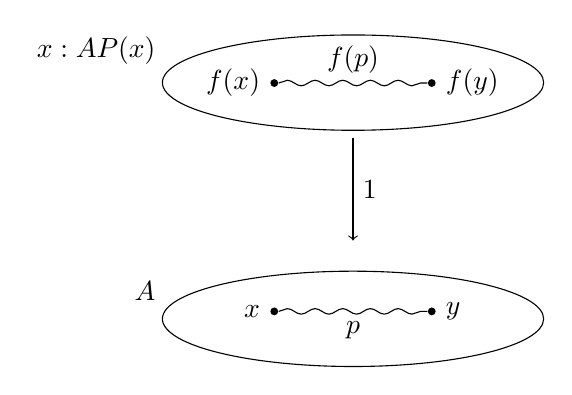
\begin{tikzpicture}[yscale=.5,xscale=2]
    \draw (0,0) arc (-90:170:8ex) node[anchor=south east] {$A$} arc (170:270:8ex);
    \draw (0,6) arc (-90:170:8ex) node[anchor=south east] {$\sm{x:A} P(x)$} arc (170:270:8ex);
    \draw[->] (0,5.8) -- node[auto] {$\proj1$} (0,3.2);
    \node[circle,fill,inner sep=1pt,label=left:{$x$}] (b1) at (-.5,1.4) {};
    \node[circle,fill,inner sep=1pt,label=right:{$y$}] (b2) at (.5,1.4) {};
    \draw[decorate,decoration={snake,amplitude=1}] (b1) -- node[auto,swap] {$p$} (b2);
    \node[circle,fill,inner sep=1pt,label=left:{$f(x)$}] (b1) at (-.5,7.2) {};
    \node[circle,fill,inner sep=1pt,label=right:{$f(y)$}] (b2) at (.5,7.2) {};
    \draw[decorate,decoration={snake,amplitude=1}] (b1) -- node[auto] {$f(p)$} (b2);
  \end{tikzpicture}
\end{center}

我们\emph{确实可以}从\cref{lem:map}得到这样的对象。
给定$f:\prd{x:A} P(x)$，我们可以令$f'(x)\defeq (x,f(x))$来定义一个非依值函数$f':A\to \sm{x:A} P(x)$，进而考虑$\ap{f'}{p} : f'(x) = f'(y)$。
由于 $\proj1 \circ f' \jdeq \idfunc[A]$，由\cref{lem:ap-functor}可得$\ap{\proj1}{\ap{f'}{p}} = p$；因此 $\ap{f'}{p}$ 确实在此意义上"位于" $p$ 的上方。
然而，仅凭 $\ap{f'}{p}$ 的\emph{类型}，并不容易看出它究竟位于 $A$ 中哪条具体道路（本例中即 $p$）的上方，而这一点有时很重要。

解决方法是使用迁移引理。
根据\cref{thm:path-lifting}，我们有一条从 $(x,u)$ 到 $(y,\trans p u)$ 的典范道路 $\mathsf{lift}(u,p)$，它位于 $p$ 的上方。
因此，任何从 $u:P(x)$ 到 $v:P(y)$ 且位于 $p$ 上方的道路，都应本质唯一地通过 $\mathsf{lift}(u,p)$ 进行分解，其分解因子是一条完全位于纤维 $P(y)$ 中、从 $\trans p u$ 到 $v$ 的道路。
因此，在相差等价的意义下，将"从 $u$ 到 $v$ 且位于 $p:x=y$ 上方的道路"定义为 $P(y)$ 中的道路 $\trans p u = v$ 是合理的。
而且，我们确实可以证明依值函数会产生这样的道路。

\begin{lem}[依值映射]\label{lem:mapdep}
  \indexdef{application!of dependent function to a path}%
  \indexdef{path!application of a dependent function to}%
  \indexdef{function!dependent!application to a path of}%
  \indexdef{action!of a dependent function on a path}%
  假设$f:\prd{x: A} P(x)$；那么我们有一个映射
  \[\apdfunc f : \prd{p:x=y}\big(\id[P(y)]{\trans p{f(x)}}{f(y)}\big).\]
\end{lem}

\begin{proof}[第一种证明]
  令$D:\prd{x,y:A} (\id{x}{y}) \to \type$为由下式定义的类型族：
  \begin{equation*}
    D(x,y,p)\defeq \trans p {f(x)}= f(y).
  \end{equation*}
  那么$D(x,x,\refl{x})$就是$\trans{(\refl{x})}{f(x)}= f(x)$。
  但由于$\trans{(\refl{x})}{f(x)}\jdeq f(x)$，我们得到$D(x,x,\refl{x})\jdeq (f(x)= f(x))$。
  因此，我们得到函数
  \begin{equation*}
    d\defeq\lam{x} \refl{f(x)}:\prd{x:A} D(x,x,\refl{x})
  \end{equation*}
  现在，道路归纳便对每个 $p:x=y$ 给出$\apdfunc f(p):\trans p{f(x)}= f(y)$。
\end{proof}

\begin{proof}[第二种证明]
  通过归纳，只需假设 $p$ 是 $\refl x$。
  但此时所求等式为$\trans{(\refl{x})}{f(x)}= f(x)$，判断成立。
\end{proof}

我们将把这种意义上"位于其他道路上方的道路"统称为\emph{依值道路（dependent paths）}。
\indexsee{dependent!path}{path, dependent}%
\index{path!dependent}%
从\cref{cha:hits}开始，它们将扮演越来越重要的角色。
在\cref{sec:computational}中我们会看到，对于少数几种特定的类型族，存在一些等价的、有时更方便的表示依值道路概念的方式。

现在回忆\cref{sec:pi-types}，非依值类型的函数 $f:A\to B$ 只是依值类型函数$f:\prd{x:A} P(x)$在 $P$ 为常值类型族（即 $P(x) \defeq B$）时的特例。
此时，$\apdfunc{f}$ 与 $\apfunc{f}$ 密切相关，这由以下引理保证：

\begin{lem}\label{thm:trans-trivial}
  如果 $P:A\to\type$ 对某个固定的 $B:\type$ 定义为 $P(x) \defeq B$，那么对于任意 $x,y:A$ 和 $p:x=y$ 以及 $b:B$，我们有一条道路
  \[ \transconst Bpb : \transfib P p b = b. \]
\end{lem}

\begin{proof}[第一种证明]
  固定一个 $b:B$，并令$D:\prd{x,y:A} (\id{x}{y}) \to \type$为由下式定义的类型族：
  \[ D(x,y,p) \defeq (\transfib P p b = b). \]
  则 $D(x,x,\refl x)$ 即$(\transfib P{\refl{x}}{b} = b)$，根据迁移的计算规则，它与 $(b=b)$ 判断相等。
  因此，我们有函数
  \[ d \defeq \lam{x} \refl{b} : \prd{x:A} D(x,x,\refl x). \]
  现在，道路归纳便给出
  \narrowequation{
    \prd{x,y:A}{p:x=y}(\transfib P p b = b)}
  类型的一个元素，如我们所愿。
\end{proof}

\begin{proof}[第二种证明]
  通过归纳，只需假设 $y$ 是 $x$ 且 $p$ 是 $\refl x$。
  但 $\transfib P {\refl x} b \jdeq b$，故此时所需证明的不过是 $b=b$，而 $\refl{b}$ 即可。
\end{proof}

因此，对于任意 $x,y:A$、$p:x=y$ 和 $f:A\to B$，通过分别与 $\transconst Bp{f(x)}$ 及其逆进行拼接，我们得到函数
\begin{align}
  \big(f(x) = f(y)\big) &\to \big(\trans{p}{f(x)} = f(y)\big)\label{eq:ap-to-apd}
  \qquad\text{and} \\
  \big(\trans{p}{f(x)} = f(y)\big) &\to \big(f(x) = f(y)\big).\label{eq:apd-to-ap}
\end{align}
实际上，这些函数是互逆的等价（在\cref{sec:basics-equivalences}将要引入的意义上），并且它们将 $\apfunc f (p)$ 与 $\apdfunc f (p)$ 联系起来。

\begin{lem}\label{thm:apd-const}
  对于 $f:A\to B$ 和 $p:\id[A]xy$，我们有
  \[ \apdfunc f(p) = \transconst B p{f(x)} \ct \apfunc f (p). \]
\end{lem}

\begin{proof}[第一种证明]
  令$D:\prd{x,y:A} (\id xy) \to \type$为由下式定义的类型族：
  \[ D(x,y,p) \defeq \big(\apdfunc f (p) = \transconst Bp{f(x)} \ct \apfunc f (p)\big). \]
  因此，我们有
  \[D(x,x,\refl x) \jdeq \big(\apdfunc f (\refl x) = \transconst B{\refl x}{f(x)} \ct \apfunc f ({\refl x})\big).\]
  但根据定义，出现在这个类型中的所有三条道路都是 $\refl{f(x)}$，所以我们有
  \[ \refl{\refl{f(x)}} : D(x,x,\refl x). \]
  因此，道路归纳便给出$\prd{x,y:A}{p:x=y} D(x,y,p)$类型的一个元素，即为所求。
\end{proof}

\begin{proof}[第二种证明]
  通过归纳，只需假设 $y$ 是 $x$ 且 $p$ 是 $\refl x$。
  此时需要证明的是$\refl{f(x)} = \refl{f(x)} \ct \refl{f(x)}$，判断成立。
\end{proof}

由于 $\apdfunc{f}$ 与 $\apfunc{f}$ 的类型不同，使用不同的记号通常会更清晰。
% We may sometimes use a notation $\apd f p$ for $\apdfunc{f}(p)$, which is similar to the notation $\ap f p$ for $\apfunc{f}(p)$.

\index{function!dependent|)}%

至此，我们希望读者已开始对基于相等类型的归纳证明有所体会。
从今往后，我们将不再同时给出两种风格的证明，而是选用最清晰、最便捷的（通常是第二种更简洁的）证明方式。
以下是关于迁移的其他几个有用引理；我们将其证明留给读者（选用任一风格均可）。

\begin{lem}\label{thm:transport-concat}
  给定 $P:A\to\type$，其中 $p:\id[A]xy$ 且 $q:\id[A]yz$，以及 $u:P(x)$，我们有
  \[ \trans{q}{\trans{p}{u}} = \trans{(p\ct q)}{u}. \]
\end{lem}

\begin{lem}\label{thm:transport-compose}
  对于函数 $f:A\to B$ 和类型族 $P:B\to\type$，以及任意的 $p:\id[A]xy$ 和 $u:P(f(x))$，我们有
  \[ \transfib{P\circ f}{p}{u} = \transfib{P}{\apfunc f(p)}{u}. \]
\end{lem}

\begin{lem}\label{thm:ap-transport}
  对于 $P,Q:A\to \type$ 和一族函数 $f:\prd{x:A} P(x)\to Q(x)$，以及任意的 $p:\id[A]xy$ 和 $u:P(x)$，我们有
  \[ \transfib{Q}{p}{f_x(u)} = f_y(\transfib{P}{p}{u}). \]
\end{lem}

\index{type!family of|)}%
\index{transport|)}

\section{同伦与等价}
\label{sec:basics-equivalences}

\index{homotopy|(defstyle}%

至此，我们已经了解了如何将相等类型 $\id[A]xy$ 视为类型 $A$ 中两个元素 $x$ 与 $y$ 之间的\emph{相等证明}、\emph{道路}或\emph{等价}。
现在，我们来探究\emph{函数}之间以及\emph{类型}之间合适的"等同"或"相同"概念。
在\cref{sec:compute-pi,sec:compute-universe}中，我们将看到同伦类型论允许我们将这些概念与相等类型的实例等同起来，但在此之前，我们需要先理解它们本身。

传统上，我们认为两个函数相同，如果它们在所有输入上取相等的值。
在"命题即类型"的解释下，这提示我们，两个（可能是依值的）函数 $f$ 和 $g$ 相同，当类型 $\prd{x:A} (f(x)=g(x))$ 是有实例的。
在同伦解释下，这个依值函数类型由\emph{连续}的道路或\emph{函子性}的等价构成，因此可视为\emph{同伦}或\emph{自然同构}的类型。\index{isomorphism!natural}
我们将采用拓扑学的术语。

\begin{defn} \label{defn:homotopy}
  设 $f,g:\prd{x:A} P(x)$ 是类型族 $P:A\to\type$ 的两个截面。
  从 $f$ 到 $g$ 的一个\define{同伦}（homotopy）
  是一个类型为
  \begin{equation*}
    (f\htpy g) \defeq \prd{x:A} (f(x)=g(x)).
  \end{equation*}
  的依值函数。
\end{defn}

注意，一个同伦并不等同于 $(f=g)$ 的一个相等证明。
不过，在\cref{sec:compute-pi}中，我们将引入一条公理，使得同伦与相等证明变得"等价"。

以下证明留给读者。

\begin{lem}\label{lem:homotopy-props}
  同伦关系在每个依值函数类型 $\prd{x:A} P(x)$ 上都是一个等价关系。
  即我们有以下类型的元素：
  \begin{gather*}
    \prd{f:\prd{x:A} P(x)} (f\htpy f)\\
    \prd{f,g:\prd{x:A} P(x)} (f\htpy g) \to (g\htpy f)\\
    \prd{f,g,h:\prd{x:A} P(x)} (f\htpy g) \to (g\htpy h) \to (f\htpy h).
  \end{gather*}
\end{lem}

% This is judgmental and is \cref{ex:composition}.
% \begin{lem}
%   Composition is associative and unital up to homotopy.
%   That is:
%   \begin{enumerate}
%   \item If $f:A\to B$ then $f\circ \idfunc[A]\htpy f\htpy \idfunc[B]\circ f$.
%   \item If $f:A\to B, g:B\to C$ and $h:C\to D$ then $h\circ (g\circ f) \htpy (h\circ g)\circ f$.
%   \end{enumerate}
% \end{lem}

\index{functoriality of functions in type theory@``functoriality'' of functions in type theory}%
\index{continuity of functions in type theory@``continuity'' of functions in type theory}%
正如类型论中的函数自动是"函子"一样，同伦也自动是\index{naturality of homotopies@``naturality'' of homotopies}%"自然变换"。
我们仅对非依值函数 $f,g:A\to B$ 陈述并证明这一点；在\cref{ex:dep-htpy-natural}中，请读者将其推广到依值函数的情形。

回忆一下，对于 $f:A\to B$ 和 $p:\id[A]xy$，我们可以记 $\ap f p$ 来表示 $\apfunc{f} (p)$。

\begin{lem}\label{lem:htpy-natural}
  假设 $H:f\htpy g$ 是函数 $f,g:A\to B$ 之间的一个同伦，并令 $p:\id[A]xy$。那么我们有
  \begin{equation*}
    H(x)\ct\ap{g}{p}=\ap{f}{p}\ct H(y).
  \end{equation*}
  我们也可以将其画成一个交换图：\index{diagram}
  \begin{align*}
    \xymatrix{
      f(x) \ar@{=}[r]^{\ap fp} \ar@{=}[d]_{H(x)} & f(y) \ar@{=}[d]^{H(y)} \\
      g(x) \ar@{=}[r]_{\ap gp} & g(y)
    }
  \end{align*}
\end{lem}

\begin{proof}
  通过归纳，只需假设 $p$ 是 $\refl x$。
  由于 $\apfunc{f}$ 和 $\apfunc g$ 在自反性上的计算，此时所需证明的是
  \[ H(x) \ct \refl{g(x)} = \refl{f(x)} \ct H(x). \]
  但由于等式两边都等于 $H(x)$，结论成立。
\end{proof}

\begin{cor}\label{cor:hom-fg}
  设 $H : f \htpy \idfunc[A]$ 是一个同伦，其中 $f : A \to A$。那么对于任意 $x : A$，我们有 \[ H(f(x)) = \ap f{H(x)}. \]
  % The above path will be denoted by $\com{H}{f}{x}$.
\end{cor}


\noindent
此处 $f(x)$ 表示 $f$ 对 $x$ 的普通函数应用，而 $\ap f{H(x)}$ 表示 $\apfunc{f}(H(x))$。


\begin{proof}
由 $H$ 的自然性，下面的道路图交换：
\begin{align*}
\xymatrix@C=3pc{
ffx \ar@{=}[r]^-{\ap f{Hx}} \ar@{=}[d]_{H(fx)} & fx \ar@{=}[d]^{Hx} \\
fx \ar@{=}[r]_-{Hx} & x
}
\end{align*}
也就是说，$\ap f{H x} \ct H x = H(f x) \ct H x$。
现在我们可以通过须接 $\opp{(H x)}$ 来消去 $H x$，从而得到
\[ \ap f{H x}
= \ap f{H x} \ct H x \ct \opp{(H x)}
= H(f x) \ct H x \ct \opp{(H x)}
= H(f x)
\]
如我们所愿（此处省略了一些结合律道路）。
\end{proof}

当然，如同函数的函子性（\cref{lem:ap-functor}），\cref{lem:htpy-natural}中的等式本身也是一条满足其自身相干律的道路，依此类推。

\index{homotopy|)}%

\index{equivalence|(}%
现在转向类型。从传统观点来看，我们可以说一个函数 $f:A\to B$ 是一个\emph{同构（isomorphism）}，如果存在一个函数 $g:B\to A$，使得两个复合 $f\circ g$ 和 $g\circ f$ 都点态相等于恒等函数；也就是说，满足 $f \circ g \htpy \idfunc[B]$ 和 $g\circ f \htpy \idfunc[A]$。
\indexsee{homotopy!equivalence}{equivalence}%
从同伦论的角度看，这应被称为\emph{同伦等价（homotopy equivalence）}；而从范畴论的角度看，则应称为\emph{（高阶）群胚的等价（equivalence of (higher) groupoids）}。
然而，在进行证明相关的数学时，
\index{mathematics!proof-relevant}%
其对应的类型
\begin{equation}
  \sm{g:B\to A} \big((f \circ g \htpy \idfunc[B]) \times (g\circ f \htpy \idfunc[A])\big)\label{eq:qinvtype}
\end{equation}
表现不佳。
例如，对于单个函数 $f:A\to B$，\eqref{eq:qinvtype} 中可能存在多个彼此不相等的居民。
（这与高阶范畴论中的一个观察密切相关：我们常常需要考虑\emph{伴随等价（adjoint equivalence）}\index{adjoint!equivalence}，而不仅仅是普通的等价。）
为此，我们转而赋予~\eqref{eq:qinvtype} 下面这个历史上准确但听起来略带贬义色彩的名字。

\begin{defn}\label{defn:quasi-inverse}
  对于函数 $f:A\to B$，$f$ 的一个\define{拟逆（quasi-inverse）}
  \indexdef{quasi-inverse}%
  \indexsee{function!quasi-inverse of}{quasi-inverse}%
  是一个三元组 $(g,\alpha,\beta)$，其中包含一个函数 $g:B\to A$ 以及两个同伦
$\alpha:f\circ g\htpy \idfunc[B]$ 和 $\beta:g\circ f\htpy \idfunc[A]$。
\end{defn}

\symlabel{qinv}
因此，~\eqref{eq:qinvtype} 就是\emph{$f$ 的拟逆构成的类型}；我们可以将其记作 $\qinv(f)$。

\begin{eg}\label{eg:idequiv}
  \index{identity!function}%
  \index{function!identity}%
  恒等函数 $\idfunc[A]:A\to A$ 有一个拟逆，就是 $\idfunc[A]$ 本身，连同由 $\alpha(y) \defeq \refl{y}$ 和 $\beta(x) \defeq \refl{x}$ 定义的同伦。
\end{eg}

\begin{eg}\label{eg:concatequiv}
  对于任意 $p:\id[A]xy$ 和 $z:A$，函数
  \begin{align*}
    (p\ct \blank)&:(\id[A]yz) \to (\id[A]xz) \qquad\text{and}\\
    (\blank \ct p)&:(\id[A]zx) \to (\id[A]zy)
  \end{align*}
  分别以 $(\opp p \ct \blank)$ 和 $(\blank \ct \opp p)$ 为拟逆；参见\cref{ex:equiv-concat}。
\end{eg}

\begin{eg}\label{thm:transportequiv}
  对于任意 $p:\id[A]xy$ 和 $P:A\to\type$，函数
  \[\transfib{P}{p}{\blank}:P(x) \to P(y)\]
  有一个拟逆 $\transfib{P}{\opp p}{\blank}$；这可由 \narrowbreak \cref{thm:transport-concat} 得出。
\end{eg}

\symlabel{basics-isequiv}\symlabel{basics:iso}
一般来说，我们仅在类型 $A$ 和 $B$ "表现得像集合"时（参见\cref{sec:basics-sets}），才使用\emph{同构（isomorphism）}一词
\index{isomorphism!of sets}
（以及类似词语，如\emph{双射（bijection）}，及相关记号 $A\cong B$）
\index{bijection}
。在这种情况下，类型~\eqref{eq:qinvtype} 不存在问题。
我们将\emph{等价（equivalence）}一词留给一个改进的概念 $\isequiv (f)$，它需满足以下性质：%


\begin{enumerate}
\item 对每个 $f:A\to B$，存在一个函数 $\qinv(f) \to \isequiv (f)$。\label{item:be1}
\item 类似地，对每个 $f$，我们有 $\isequiv (f) \to \qinv(f)$；因此二者是逻辑等价的（参见\cref{sec:pat}）。\label{item:be2}
\item 对于任意两个居民 $e_1,e_2:\isequiv(f)$，有 $e_1=e_2$。\label{item:be3}
\end{enumerate}


在\cref{cha:equivalences}中我们将会看到，有许多不同的 $\isequiv(f)$ 定义都满足这三条性质，但它们彼此都是等价的。
现在，为了让读者相信这样的定义是存在的，我们仅提及其中最简单的一个：
\begin{equation}\label{eq:isequiv-invertible}
  \isequiv(f) \;\defeq\;
  \Parens{\sm{g:B\to A} (f\circ g \htpy \idfunc[B])}
  \times
  \Parens{\sm{h:B\to A} (h\circ f \htpy \idfunc[A])}.
\end{equation}
我们现在就可以证明这个定义满足性质~\ref{item:be1}和~\ref{item:be2}。
要定义一个函数 $\qinv(f) \to \isequiv (f)$ 很容易：将 $(g,\alpha,\beta)$ 映到 $(g,\alpha,g,\beta)$ 即可。
反之，给定 $(g,\alpha,h,\beta)$，令 $\gamma$ 为如下的复合同伦
\[ g \overset{\beta}{\htpy} h\circ f\circ g \overset{\alpha}{\htpy} h, \]
即 $\gamma(x) \defeq \opp{\beta(g(x))} \ct \ap{h}{\alpha(x)}$。
现在，由 $\beta'(x) \defeq \gamma(f(x)) \ct \beta(x)$ 定义 $\beta':g\circ f\htpy \idfunc[A]$。
则有 $(g,\alpha,\beta'):\qinv(f)$。

对此定义证明性质~\ref{item:be3} 也不难，但需要先确定 Cartesian 积和依值对类型的相等类型，我们将在\cref{sec:compute-cartprod,sec:compute-sigma}中讨论这一点。
因此，我们也将其推迟；详见\cref{sec:biinv}。
此刻，主要应理解的是：存在一个表现良好的类型，我们可以将其读作"$f$ 是一个等价"；并且，我们可以通过给出 $f$ 的一个拟逆来证明 $f$ 是一个等价。
在实践中，这是证明一个函数是等价的最常用方法。

依照证明相关的理念，
\index{mathematics!proof-relevant}%
从 $A$ 到 $B$ 的一个\emph{等价（equivalence）}被定义为一个函数 $f:A\to B$ 连同 $\isequiv (f)$ 的一个居民，即它为等价的证明。
我们记 $(\eqv A B)$ 为从 $A$ 到 $B$ 的等价构成的类型，即类型
\begin{equation}\label{eq:eqv}
  (\eqv A B) \defeq \sm{f:A\to B} \isequiv(f).
\end{equation}
上述性质~\ref{item:be3} 保证了，如果两个等价作为函数是相等的（即它们作为 $A\to B$ 中的底层元素是相等的），那么它们作为等价也是相等的（参见 \cref{sec:compute-sigma}）。
因此，我们常常滥用记号，模糊等价与其底层函数之间的区别。
例如，如果我们有一个函数 $f:A\to B$，并且知道 $e:\isequiv(f)$，我们可以写成 $f:\eqv A B$，而不是 $\tup{f}{e}$。
反之，如果我们有一个等价 $g:\eqv A B$，那么给定 $a:A$，我们可以直接写 $g(a)$，而不是 $(\proj1 g)(a)$。

最后，我们指出如下观察：

\begin{lem}\label{thm:equiv-eqrel}
  类型等价是 \type 上的一个等价关系。
  具体来说：
  \begin{enumerate}
  \item 对任意 $A$，恒等函数 $\idfunc[A]$ 是一个等价；因此 $\eqv A A$。
  \item 对任意 $f:\eqv A B$，我们有一个等价 $f^{-1} : \eqv B A$。
  \item 对任意 $f:\eqv A B$ 和 $g:\eqv B C$，我们有 $g\circ f : \eqv A C$。
  \end{enumerate}
\end{lem}

\begin{proof}
  恒等函数显然是自身的拟逆；因此它是一个等价。

  如果 $f:A\to B$ 是一个等价，那么它有一个拟逆，设其为 $f^{-1}:B\to A$。
  则 $f$ 也是 $f^{-1}$ 的一个拟逆，所以 $f^{-1}$ 是一个 $B\to A$ 的等价。

  最后，给定 $f:\eqv A B$ 和 $g:\eqv B C$，设其拟逆分别为 $f^{-1}$ 和 $g^{-1}$，则对于任意 $a:A$，我们有 $f^{-1} g^{-1} g f a = f^{-1} f a = a$，而对于任意 $c:C$，我们有 $g f f^{-1} g^{-1} c = g g^{-1} c = c$。
  因此 $f^{-1} \circ g^{-1}$ 是 $g\circ f$ 的一个拟逆，从而 $g\circ f$ 是一个等价。
\end{proof}

\index{equivalence|)}%

\section{类型形成子的高阶群胚结构}
\label{sec:computational}

在 \cref{cha:typetheory} 中，我们介绍了多种形成新类型的方法：Cartesian 积、不交并、依值积、依值和等等。
在 \cref{sec:equality,sec:functors,sec:fibrations} 中，我们看到同伦类型论中的\emph{所有}类型都表现得像空间或高阶群胚。
本章剩余部分的目标是，在 \cref{cha:typetheory} 所定义的特定类型的案例中，明确这种高阶结构是如何表现的。

事实证明，对于许多类型 $A$，其相等类型 $\id[A]xy$ 可以用构造 $A$ 时所用的数据，在等价的意义下刻画出来。
例如，如果 $A$ 是一个 Cartesian 积 $B\times C$，并且 $x\jdeq (b,c)$，$y\jdeq(b',c')$，那么我们有一个等价
\begin{equation}\label{eq:prodeqv}
  \eqv{\big((b,c)=(b',c')\big)}{\big((b=b')\times (c=c')\big)}.
\end{equation}
用更传统的语言来说，两个有序对相等当且仅当它们的各分量分别相等（但等价~\eqref{eq:prodeqv} 所说的比这更多）。
相等类型的高阶结构也可以用这些等价来表达；例如，拼接两个关于有序对的相等性，对应于各分量上的逐对拼接。

类似地，当一个类型族 $P:A\to\type$ 是使用 \cref{cha:typetheory} 中的类型形成规则逐纤维地构建起来时，操作 $\transfib{P}{p}{\blank}$ 可以在同伦的意义下，根据构建 $P$ 所用数据的相应操作来刻画。
例如，如果 $P(x) \jdeq B(x)\times C(x)$，那么我们有
\[\transfib{P}{p}{(b,c)} = \big(\transfib{B}{p}{b},\transfib{C}{p}{c}\big).\]

最后，类型形成规则也具有函子性，并且如果一个函数 $f$ 是基于这种函子性构建的，那么 $\apfunc f$ 和 $\apdfunc f$ 这两个操作，可以根据构造 $f$ 所用数据的相应操作来计算。
例如，如果 $g:B\to B'$ 且 $h:C\to C'$，并且我们通过 $f(b,c)\defeq (g(b),h(c))$ 来定义 $f:B\times C \to B'\times C'$，那么模掉等价~\eqref{eq:prodeqv}，我们可以将 $\apfunc f$ 与 "$(\apfunc g,\apfunc h)$" 等同。

接下来的几节（\crefrange{sec:compute-cartprod}{sec:compute-nat}）将致力于为所有基本的类型形成规则陈述并证明这类定理，每个基本类型形成子对应一节。
在这里，我们遇到了当前可用的类型理论中一个表面上的不足之处；
正如在后续章节中将会明确的那样，如果这些关于相等类型、传输等等的刻画是\emph{判断相等性}\index{judgmental equality}，似乎会更方便且更直观。
然而，在 \cref{cha:typetheory} 所介绍的理论中，相等类型由其归纳原理为所有类型统一地定义，因此我们不能对不同的类型将它们"重新定义"为不同的东西。
因此，本章将要讨论的针对特定类型的刻画，大多是\emph{定理}，需要我们去发现和证明——如果可能的话。

实际上，\cref{cha:typetheory} 所描述的类型论不足以证明两类类型形成子——$\Pi$-类型与宇宙——所期望的那些定理。
正因如此，我们不得不向类型论中引入公理，以使这些"定理"成立。
从类型论的角度看，\emph{公理}（axiom，参见~\cref{sec:axioms}）是一个被声明居住于某个特定类型的"原子"元素；除了其所属类型的规则之外，没有任何其他规则支配其行为。
\index{axiom!versus rules}%

\index{function extensionality}%
\indexsee{extensionality, of functions}{function extensionality}
\index{univalence axiom}%
关于 $\Pi$-类型（\cref{sec:compute-pi}）的公理对于类型论研究者来说并不陌生：它被称为\emph{函数外延性}，其内容（粗略地说）是：如果两个函数在\cref{sec:basics-equivalences}的意义下是同伦的，那么它们相等。
然而，关于宇宙（\cref{sec:compute-universe}）的公理，则是同伦类型论中由 Voevodsky 提出的新贡献：它被称为\emph{泛等公理}，其内容（粗略地说）是：如果两个类型在\cref{sec:basics-equivalences}的意义下是等价的，那么它们相等。
我们已在导论中提到过这条公理；它将在本书中发挥重要作用。%
\footnote{我们选择将这些原理作为公理引入，但也存在其他可能的方式来构造一套使之成立的类型论。
  详见本章注记。}

需要特别注意的是，并非\emph{所有}的相等类型都能通过对类型构造进行归纳来"确定"。
反例包括大多数非平凡的高阶归纳类型（参见\cref{cha:hits,cha:homotopy}）。
例如，计算类型 $\Sn^n$（参见\cref{sec:circle}）的相等类型，就相当于计算球面的高阶同伦群——这是代数拓扑学中一个深刻而重要的研究领域。

\section{Cartesian 积类型}
\label{sec:compute-cartprod}

\index{type!product|(}%
给定类型 $A$ 和 $B$，考虑它们的 Cartesian 积类型 $A \times B$。
对于任意元素 $x,y:A\times B$ 以及一条道路$p:\id[A\times B]{x}{y}$，由函子性我们可以提取出道路$\ap{\proj1}p:\id[A]{\proj1(x)}{\proj1(y)}$与$\ap{\proj2}p:\id[B]{\proj2(x)}{\proj2(y)}$。
于是，我们得到一个函数
\begin{equation}\label{eq:path-prod}
  (\id[A\times B]{x}{y}) \to (\id[A]{\proj1(x)}{\proj1(y)}) \times (\id[B]{\proj2(x)}{\proj2(y)}).
\end{equation}

\begin{thm}\label{thm:path-prod}
  对于任意的 $x$ 和 $y$，函数~\eqref{eq:path-prod}是一个等价。
\end{thm}

从逻辑的角度看，这意味着两个序对相等，当且仅当它们逐个分量相等。
从范畴论的角度看，这意味着积群胚中的态射就是态射对。
从同伦论的角度看，这意味着积空间中的道路就是道路对。

\begin{proof}
  我们需要构造一个方向相反的函数：
  \begin{equation}
    (\id[A]{\proj1(x)}{\proj1(y)}) \times (\id[B]{\proj2(x)}{\proj2(y)}) \to (\id[A\times B]{x}{y}). \label{eq:path-prod-inverse}
  \end{equation}
  根据 Cartesian 积的归纳规则，我们可以假设 $x$ 和 $y$ 都是序对，即对某个 $a,a':A$ 和 $b,b':B$，有 $x\jdeq (a,b)$ 且 $y\jdeq (a',b')$。
  此时，我们需要的是一个形如
  \begin{equation*}
    (\id[A]{a}{a'}) \times (\id[B]{b}{b'}) \to \big(\id[A\times B]{(a,b)}{(a',b')}\big).
  \end{equation*}
  的函数。
  现在，通过对其定义域中的 Cartesian 积进行归纳，我们可以假设给定了 $p:a=a'$ 和 $q:b=b'$。
  接着，通过两次道路归纳，我们可以假设 $a\jdeq a'$ 且 $b\jdeq b'$，并且 $p$ 和 $q$ 都是自反性。
  但在这种情况下，我们有$(a,b)\jdeq(a',b')$，因此我们可以将输出也取为自反性。

  接下来需要证明~\eqref{eq:path-prod-inverse}是~\eqref{eq:path-prod}的拟逆。
  这是一系列简单的归纳，但必须按正确的顺序进行。

  在一个方向上，我们从$r:\id[A\times B]{x}{y}$出发。
  我们首先对 $r$ 作道路归纳，以便假设 $x\jdeq y$ 且 $r$ 是自反性。
  此时，由于 $\apfunc{\proj1}$ 和 $\apfunc{\proj2}$ 是通过道路归纳定义的，~\eqref{eq:path-prod}将 $r\jdeq \refl{x}$ 映射到序对$(\refl{\proj1x},\refl{\proj2x})$。
  现在，通过对 $x$ 进行归纳，可假设 $x\jdeq (a,b)$，于是这个序对就是 $(\refl a, \refl b)$。
  因此，根据定义，~\eqref{eq:path-prod-inverse}将其映射到 $\refl{(a,b)}$，这（在我们当前的假设下）就是 $r$。

  在另一个方向上，如果我们从$s:(\id[A]{\proj1(x)}{\proj1(y)}) \times (\id[B]{\proj2(x)}{\proj2(y)})$出发，那么首先对 $x$ 和 $y$ 进行归纳，假设它们是序对 $(a,b)$ 和 $(a',b')$；然后对$s:(\id[A]{a}{a'}) \times (\id[B]{b}{b'})$进行归纳，将其归约为序对 $(p,q)$，其中 $p:a=a'$ 且 $q:b=b'$。
  接着，对 $p$ 和 $q$ 进行归纳，可以假设它们分别是自反性 $\refl a$ 和 $\refl b$；在这种情况下，~\eqref{eq:path-prod-inverse}给出 $\refl{(a,b)}$，然后~\eqref{eq:path-prod}再给出$(\refl a,\refl b)\jdeq (p,q)\jdeq s$。
\end{proof}

特别地，我们证明了~\eqref{eq:path-prod}有一个逆~\eqref{eq:path-prod-inverse}，我们可以将其记作
\symlabel{defn:pairpath}
\[
\pairpath : (\id{\proj{1}(x)}{\proj{1}(y)}) \times (\id{\proj{2}(x)}{\proj{2}(y)}) \to (\id x y).
\]
注意，它的一个特例给出了积类型的命题唯一性原理\index{uniqueness!principle, propositional!for product types}：$z = (\proj1(z),\proj2(z))$。

不妨把 \pairpath 看作 $\id x y$ 的一个\emph{构造子}或\emph{引入规则}，这就好比 $A\times B$ 类型本身的"配对"构造子，它在给定 $a:A$ 和 $b:B$ 时构造出序对 $(a,b)$。
从这个视角看，~\eqref{eq:path-prod}的两个分量：
\begin{align*}
  \projpath{1} &: (\id{x}{y}) \to (\id{\proj{1}(x)}{\proj{1} (y)})\\
  \projpath{2} &: (\id{x}{y}) \to (\id{\proj{2}(x)}{\proj{2} (y)})
\end{align*}
就是\emph{消去}规则。
类似地，见证~\eqref{eq:path-prod-inverse}为~\eqref{eq:path-prod}之拟逆的两条同伦，分别由\emph{命题计算规则}：
\index{computation rule!propositional!for identities between pairs}%
\begin{align*}
  {\projpath{1}{(\pairpath(p, q)})}
  &= %_{(\id{\proj{1} x}{\proj{1} y})}
  {p} \\
  {\projpath{2}{(\pairpath(p,q)})}
  &= %_{(\id{\proj{2} x}{\proj{2} y})}
  {q}
\end{align*}
（针对 $p:\id{\proj{1} x}{\proj{1} y}$ 和 $q:\id{\proj{2} x}{\proj{2} y}$）
以及一条\emph{命题唯一性原理}：
\index{uniqueness!principle, propositional!for identities between pairs}%
\[
\id{r}{\pairpath(\projpath{1} (r), \projpath{2} (r)) }
\qquad\text{for } r : \id[A \times B] x y.
\]
构成。

我们也可以按分量刻画 $A\times B$ 中道路的自反性、逆和复合：
\begin{align*}
  {\refl{(z : A \times B)}}
  &= {\pairpath (\refl{\proj{1} z},\refl{\proj{2} z})} \\
  {\opp{p}}
  &= {\pairpath \big(\opp{\projpath{1} (p)},\, \opp{\projpath{2} (p)}\big)} \\
  {{p \ct q}}
  &= {\pairpath \big({\projpath{1} (p)} \ct {\projpath{1} (q)},\,{\projpath{2} (p)} \ct {\projpath{2} (q)}\big)}.
\end{align*}
或者，换种写法：
\begin{alignat*}{2}
  \projpath{i}(\refl{(z : A \times B)}) &= \refl{\proj{i} z} &\qquad (i=1,2)\\
  \pairpath(\opp p, \opp q) &= \opp{\pairpath(p,q)}\\
  \pairpath(p\ct q, p'\ct q') &= \pairpath(p,p') \ct \pairpath(q,q').
\end{alignat*}
所有这些等式都可以这样得到：先对给定的道路作道路归纳，然后归结为自反性。
对于 \cref{sec:equality} 中讨论的其余高阶群胚结构，这一点同样成立，尽管这会逐渐变得繁琐——因为需要插入足够多其他的一致性道路，才能写出一个能通过类型检查的等式。
例如，如果我们用 $\ctassoc(p,q,r)$ 表示 \cref{thm:omg}\ref{item:omg4} 中道路的逆，而用 $\pairct(p,q,p',q')$ 表示上面最后显示的那条道路，那么对于任何具有适当类型的 $u,v,z,w:A\times B$ 和 $p,q,r,p',q',r'$，我们有
\begin{equation*}
  \begin{array}{l}
    \pairct(p\ct q, r, p'\ct q', r') \\
    \ct\;  (\pairct(p,q,p',q') \rightwhisker \pairpath(r,r')) \\
    \ct\;  \ctassoc(\pairpath(p,p'),\pairpath(q,q'),\pairpath(r,r'))\\
    =
    \begin{array}[t]{l}
      \apfunc{\pairpath}({\pairpath(\ctassoc(p,q,r),\ctassoc(p',q',r'))})\\
      \ct\; \pairct(p, q\ct r, p', q'\ct r')\\
      \ct\; (\pairpath(p,p') \leftwhisker \pairct(q,r,q',r')).
    \end{array}
  \end{array}
\end{equation*}
幸运的是，我们永远不需要使用任何这类高维一致性。

\index{transport!in product types}%
我们现在考虑在类型族的逐点积上的传输。
给定类型族 $ A, B : Z \to \type$，我们略滥用记号，用 $A\times B:Z\to\type$ 表示由 $(A\times B)(z) \defeq A(z) \times B(z)$ 定义的类型族。
现在给定 $p : \id[Z]{z}{w}$ 和 $x : A(z) \times B(z)$，我们可以把 $x$ 沿着 $p$ 传输，从而得到 $A(w)\times B(w)$ 中的一个元素。

\begin{thm}\label{thm:trans-prod}
  在上述情形下，我们有
  \[
  \id[A(w) \times B(w)]
  {\transfib{A\times B}px}
  {(\transfib{A}{p}{\proj{1}x}, \transfib{B}{p}{\proj{2}x})}.
  \]
\end{thm}

\begin{proof}
  通过对 $p$ 作道路归纳，我们可以假设 $p$ 是自反性，此时我们有
  \begin{align*}
    \transfib{A\times B}px&\jdeq x\\
    \transfib{A}{p}{\proj{1}x}&\jdeq \proj1x\\
    \transfib{B}{p}{\proj{2}x}&\jdeq \proj2x.
  \end{align*}
  因此，只需证明 $x = (\proj1 x, \proj2x)$。
  但这就是积类型的命题唯一性原理，而如前文所述，它可由 \cref{thm:path-prod} 推出。
\end{proof}

最后，我们考虑 $\apfunc{}$ 在 Cartesian 积下的函子性。
假设给定类型 $A,B,A',B'$ 以及函数 $g:A\to A'$ 和 $h:B\to B'$；那么我们可以通过 $f(x) \defeq (g(\proj1x),h(\proj2x))$ 定义一个函数 $f:A\times B\to A'\times B'$。

\begin{thm}\label{thm:ap-prod}
  在上述情形下，给定 $x,y:A\times B$ 以及 $p:\proj1x=\proj1y$ 和 $q:\proj2x=\proj2y$，我们有
  \[ \id[(f(x)=f(y))]{\ap{f}{\pairpath(p,q)}} {\pairpath(\ap{g}{p},\ap{h}{q})}. \]
\end{thm}

\begin{proof}
  首先注意，上面的方程是良类型的。
  一方面，由于 $\pairpath(p,q):x=y$，我们有 $\ap{f}{\pairpath(p,q)}:f(x)=f(y)$。
  另一方面，由于 $\proj1(f(x))\jdeq g(\proj1x)$ 与 $\proj2(f(x))\jdeq h(\proj2x)$，我们也有 $\pairpath(\ap{g}{p},\ap{h}{q}):f(x)=f(y)$。

  现在，通过归纳，我们可以假设 $x\jdeq(a,b)$ 且 $y\jdeq(a',b')$，此时有 $p:a=a'$ 和 $q:b=b'$。
  于是，再通过道路归纳，我们可以假设 $p$ 和 $q$ 都是自反性，此时所求等式判断性地成立。
\end{proof}

\index{type!product|)}%

\section{\texorpdfstring{$\Sigma$}{Σ}-类型}
\label{sec:compute-sigma}

\index{type!dependent pair|(}%
设 $A$ 为一个类型，$P:A\to\type$ 为一个类型族。
回忆一下，$\Sigma$-类型，或称依值对类型，$\sm{x:A} P(x)$ 是 Cartesian 积类型的一种推广。
因此，我们预期它的高阶群胚结构也是对前一节内容的推广。
特别地，它的道路应当由一对道路组成，但要给出这些道路的正确类型，还需稍加思考。

假设我们在 $\sm{x:A}P(x)$ 中有一条道路 $p:w=w'$。
那么我们会得到 $\ap{\proj{1}}{p}:\proj{1}(w)=\proj{1}(w')$。
然而，我们不能直接问 $\proj{2}(w)$ 是否等于 $\proj{2}(w')$，因为它们不必处于同一个类型中。
但是，我们可以沿着道路 $\ap{\proj{1}}{p}$ 对 $\proj{2}(w)$ 进行传输\index{transport}，这确实能给出一个与 $\proj{2}(w')$ 类型相同的元素。
通过道路归纳，我们确实可以得到一条道路 $\trans{\ap{\proj{1}}{p}}{\proj{2}(w)}=\proj{2}(w')$。

回忆在 \cref{lem:mapdep} 之前的讨论，等式
\narrowequation{
  \trans{\ap{\proj{1}}{p}}{\proj{2}(w)}=\proj{2}(w')
}
可以看作是从 $\proj2(w)$ 到 $\proj2(w')$ 且居于 $A$ 中道路 $\ap{\proj1}{p}$ 之上的道路的类型。
\index{fibration}%
\index{total!space}%
因此，全空间中的一条道路 $w=w'$ 决定——且被决定于——$A$ 中的一条道路 $p:\proj1(w)=\proj1(w')$ 连同一条从 $\proj2(w)$ 到 $\proj2(w')$ 且居于 $p$ 之上的道路。这看来是合理的。

\begin{rmk}\label{rmk:sigma-equality-extraction}
  注意，如果我们有 $x:A$ 和 $u,v:P(x)$ 使得 $(x,u)=(x,v)$，这并不能推出 $u=v$——反例可见 \cref{ex:sigma-eq-components-neq}。
  我们所能得出的结论仅仅是：存在 $p:x=x$ 使得 $\trans p u = v$。
  这一点常常让刚接触类型论的人感到困惑，但从拓扑的观点来看却很自然：在纤维化的全空间中，两个恰好位于同一纤维内的点之间存在道路 $(x,u)=(x,v)$，这一事实并不意味着存在一条完全\emph{位于}该纤维内部的道路 $u=v$。
\end{rmk}

下面的定理说明这个过程也可以反过来。
由于它是 \cref{thm:path-prod} 的直接推广，我们在此就写得简略一些。

\begin{thm}\label{thm:path-sigma}
假设 $P:A\to\type$ 是类型 $A$ 上的类型族，且令 $w,w':\sm{x:A}P(x)$。那么存在等价
\begin{equation*}
\eqvspaced{(w=w')}{\dsm{p:\proj{1}(w)=\proj{1}(w')} \trans{p}{\proj{2}(w)}=\proj{2}(w')}.
\end{equation*}
\end{thm}

\begin{proof}
我们定义函数
\begin{equation*}
f : \prd{w,w':\sm{x:A}P(x)} (w=w') \to \dsm{p:\proj{1}(w)=\proj{1}(w')} \trans{p}{\proj{2}(w)}=\proj{2}(w')
\end{equation*}
由道路归纳给出，其中
\begin{equation*}
f(w,w,\refl{w})\defeq(\refl{\proj{1}(w)},\refl{\proj{2}(w)}).
\end{equation*}
我们要证明 $f$ 是一个等价。

反过来，我们定义
\begin{narrowmultline*}
  g : \prd{w,w':\sm{x:A}P(x)}
      \Parens{\sm{p:\proj{1}(w)=\proj{1}(w')}\trans{p}{\proj{2}(w)}=\proj{2}(w')}
      \to
      \narrowbreak
      (w=w')
\end{narrowmultline*}
通过首先对 $w$ 和 $w'$ 进行归纳，将其分别拆分为 $(w_1,w_2)$ 和
$(w_1',w_2')$，因此只需证明
\begin{equation*}
\Parens{\sm{p:w_1 = w_1'}\trans{p}{w_2}=w_2'} \to ((w_1,w_2)=(w_1',w_2')).
\end{equation*}
接下来，给定一对 $\sm{p:w_1 = w_1'}\trans{p}{w_2}=w_2'$，我们可以使用 $\Sigma$-归纳得到 $p : w_1 = w_1'$ 和 $q :
\trans{p}{w_2}=w_2'$。对 $p$ 进行归纳，我们有 $q :
\trans{(\refl{w_1})}{w_2}=w_2'$，此时只需证明
$(w_1,w_2)=(w_1,w_2')$。但 $\trans{(\refl{w_1})}{w_2} \jdeq w_2$，所以对 $q$ 进行归纳就将目标化为
$(w_1,w_2)=(w_1,w_2)$，而这可以通过 $\refl{(w_1,w_2)}$ 来证明。

接着我们证明对于所有 $w$、$w'$ 和 $r$ 都有 $f(g(r))=r$，其中 $r$ 的类型为
\[\dsm{p:\proj{1}(w)=\proj{1}(w')} (\trans{p}{\proj{2}(w)}=\proj{2}(w')).\]
首先，如 $g$ 的定义中那样，通过配对归纳拆开 $w$、$w'$ 和 $r$，然后使用两次道路归纳将 $r$ 的两个分量都归约为 \refl{}。于是只需证明
$f (g(\refl{w_1},\refl{w_2})) = (\refl{w_1},\refl{w_2})$，而由定义可知这成立。类似地，为证明对所有 $w$、$w'$ 和 $p : w = w'$ 都有 $g(f(p))=p$，我们可以对 $p$ 做道路归纳，然后做配对归纳以拆开 $w$，此时只需证明
$g(f (\refl{(w_1,w_2)})) = \refl{(w_1,w_2)}$，而这由定义即得。

因此，$f$ 有一个拟逆，从而是一个等价。
\end{proof}

正如在 Cartesian 积的情形中所做的那样，我们可以推出一个命题唯一性原理作为特例。

\begin{cor}\label{thm:eta-sigma}
  \index{uniqueness!principle, propositional!for dependent pair types}%
  对于 $z:\sm{x:A} P(x)$，我们有 $z = (\proj1(z),\proj2(z))$。
\end{cor}

\begin{proof}
  我们有 $\refl{\proj1(z)} : \proj1(z) = \proj1(\proj1(z),\proj2(z))$，故由 \cref{thm:path-sigma}，只需展示一条道路 $\trans{(\refl{\proj1(z)})}{\proj2(z)} = \proj2(\proj1(z),\proj2(z))$。
  但等式两边都判断相等于 $\proj2(z)$。
\end{proof}

类似于二元 Cartesian 积的情形，我们可以将
\cref{thm:path-sigma} 的逆向
视为引入形式（\pairpath{}{}），正向视为
消去形式（\projpath{1} 和 \projpath{2}），而该等价则给出了这些形式的命题计算规则和唯一性原理。

注意，\cref{thm:path-lifting} 中定义的提升道路 $\mathsf{lift}(u,p)$（即 $p:x=y$ 在 $u:P(x)$ 处的提升）可以等同于引入形式的特例
\[\pairpath(p,\refl{\trans p u}):(x,u) = (y,\trans p u).\]
\index{transport!in dependent pair types}%
它出现在关于 transport 在 $\Sigma$-类型上作用的定理陈述中，这也是二元 Cartesian 积情形的推广：

\begin{thm}\label{transport-Sigma}
  假设我们有类型族
  %
  \begin{equation*}
    P:A\to\type
    \qquad\text{and}\qquad
    Q:\Parens{\sm{x:A} P(x)}\to\type.
  \end{equation*}
  %
  那么我们可以构造 $A$ 上由下式定义的类型族
  \begin{equation*}
    x \mapsto \sm{u:P(x)} Q(x,u).
  \end{equation*}
  对任意道路 $p:x=y$ 和任意 $(u,z):\sm{u:P(x)} Q(x,u)$，我们有
  \begin{equation*}
    \trans{p}{u,z}=\big(\trans{p}{u},\,\trans{\pairpath(p,\refl{\trans pu})}{z}\big).
  \end{equation*}
\end{thm}

\begin{proof}
直接由道路归纳即得。
\end{proof}

我们把 \cref{thm:ap-prod} 的推广（参见 \cref{ex:ap-sigma}）的陈述和证明留给读者，并请读者逐分量地刻画 $\Sigma$-类型的自反性、逆和复合。

\index{type!dependent pair|)}%

\section{单位类型}
\label{sec:compute-unit}

\index{type!unit|(}%
平凡的情形有时也很重要，所以我们简要提一下单位类型~\unit。

\begin{thm}\label{thm:path-unit}
  对任意 $x,y:\unit$，我们有 $\eqv{(x=y)}{\unit}$。
\end{thm}

这个证明一开始可能会让人想先对 $x$ 和 $y$ 进行 $\unit$-归纳，从而将问题化为 $\eqv{(\ttt=\ttt)}{\unit}$。
但这样一来我们就会卡住，因为我们无法对 $p:\ttt=\ttt$ 进行道路归纳。
因此，我们转而尽可能一般地处理 $x$ 和 $y$，只在最后才通过归纳将它们归约为 $\ttt$。

\begin{proof}
  定义一个从 $(x=y)$ 到 $\unit$ 的函数是容易的：只需将所有元素都映到 $\ttt$。
  反过来，对于任意 $x,y:\unit$，由归纳法可以假设 $x\jdeq \ttt\jdeq y$。
  此时我们有 $\refl{\ttt}:x=y$，这就给出了一个常值函数 $\unit\to(x=y)$。

  为了证明这两个函数互逆，首先考虑一个元素 $u:\unit$。
  我们可以假设 $u\jdeq\ttt$，而这正是复合函数 $\unit \to (x=y)\to\unit$ 作用在 $u$ 上的结果。

  另一方面，给定 $p:x=y$。
  由道路归纳，我们可以假设 $x\jdeq y$ 且 $p$ 就是 $\refl x$。
  接着我们可以假设 $x$ 就是 $\ttt$，此时复合函数 $(x=y) \to \unit\to(x=y)$ 将 $p$ 映到 $\refl x$，也就是映回 $p$ 本身。
\end{proof}

因此，$\unit$ 的任意两个元素都是相等的。
我们将其留给读者，以引入规则、消去规则、计算规则和唯一性规则的形式表述此等价。
\index{transport!in unit type}%
$\unit$ 的 transport 引理就是常值类型族（\cref{thm:trans-trivial}）的 transport 引理。

\index{type!unit|)}%

\section{\texorpdfstring{$\Pi$}{Π}-类型与函数外延性公理}
\label{sec:compute-pi}

\index{type!dependent function|(}%
\index{type!function|(}%
\index{homotopy|(}%
给定一个类型 $A$ 和一个类型族 $B : A \to \type$，考虑依值函数类型 $\prd{x:A}B(x)$。
我们期望，在 $\prd{x:A} B(x)$ 中从 $f$ 到 $g$ 的道路类型 $f=g$，等价于逐点道路的类型：\index{pointwise!equality of functions}
\begin{equation}
  \eqvspaced{(\id{f}{g})}{\Parens{\prd{x:A} (\id[B(x)]{f(x)}{g(x)})}}.\label{eq:path-forall}
\end{equation}
从传统视角看，这意味着：两个在每个点上都相等的函数，作为函数也是相等的。
\index{continuity of functions in type theory@``continuity'' of functions in type theory}%
从拓扑视角看，这意味着：函数空间中的一条道路，等同于一个连续同伦。
\index{functoriality of functions in type theory@``functoriality'' of functions in type theory}%
而从范畴视角看，这意味着：函子范畴中的一个同构，就是一个自然的同构族。

然而，与前几节的情况不同，\cref{cha:typetheory} 中给出的基础类型论并不足以证明~\eqref{eq:path-forall}。
我们所能说的只是：存在某个函数
\begin{equation}\label{eq:happly}
  \happly : (\id{f}{g}) \to \prd{x:A} (\id[B(x)]{f(x)}{g(x)})
\end{equation}
它可以由道路归纳容易地定义。
因此，暂时假定：

\begin{axiom}[函数外延性]\label{axiom:funext}
  \indexsee{axiom!function extensionality}{function extensionality}%
  \indexdef{function extensionality}%
  对于任何 $A$、$B$、$f$ 和 $g$，函数~\eqref{eq:happly} 是一个等价。
\end{axiom}

我们将在后续章节中看到，这个公理既能从泛等性（参见 \cref{sec:compute-universe,sec:univalence-implies-funext}）推出，也能从区间类型（参见 \cref{sec:interval} 与 \cref{ex:funext-from-interval}）推出。

特别地，\cref{axiom:funext} 蕴含了~\eqref{eq:happly} 有一个拟逆
\[
\funext : \Parens{\prd{x:A} (\id{f(x)}{g(x)})} \to {(\id{f}{g})}.
\]
这个函数也常被称为"函数外延性"。
正如我们在 \cref{sec:compute-cartprod} 中对 $\pairpath$ 所做的那样，我们可以将 $\funext$ 视为类型 $\id f g$ 的一个\emph{引入规则}。
从这个视角看，$\happly$ 就是\emph{消去规则}，而那些见证 $\funext$ 作为 $\happly$ 之拟逆的同伦，则成为一个命题计算规则\index{computation rule!propositional!for identities between functions}
\[
\id{\happly({\funext{(h)}},x)}{h(x)} \qquad\text{for }h:\prd{x:A} (\id{f(x)}{g(x)})
\]
和一个命题唯一性原理\index{uniqueness!principle!for identities between functions}：
\[
\id{p}{\funext (x \mapsto \happly(p,{x}))} \qquad\text{for } p: \id f g.
\]

我们也可以计算 $\Pi$-类型中的恒等、逆与复合；它们简单地由逐点运算给出：\index{pointwise!operations on functions}
\begin{align*}
\refl{f} &= \funext(x \mapsto \refl{f(x)}) \\
\opp{\alpha} &= \funext (x \mapsto \opp{\happly (\alpha,x)})  \\
{\alpha} \ct \beta &= \funext (x \mapsto {\happly({\alpha},x) \ct \happly({\beta},x)}).
\end{align*}
第一个等式由 $\happly$ 的定义可得，第二、第三个则是简单的道路归纳。

由于当 $B$ 不依赖于 $x$ 时，非依值函数类型 $A\to B$ 是依值函数类型 $\prd{x:A} B(x)$ 的特例，上述所有讨论同样适用于非依值情形。
\index{transport!in function types}%
不过，在非依值情形下，transport 的规则要稍微简单一些。
给定一个类型 $X$、一条道路 $p:\id[X]{x_1}{x_2}$、两个类型族 $A,B:X\to \type$，以及一个函数 $f : A(x_1) \to B(x_1)$，我们有
\begin{align}\label{eq:transport-arrow}
  \transfib{A\to B}{p}{f} &=
  \Big(x \mapsto \transfib{B}{p}{f(\transfib{A}{\opp p}{x})}\Big)
\end{align}
其中 $A\to B$（滥用记号）表示由下式定义的类型族 $X\to \type$：
\[(A\to B)(x) \defeq (A(x)\to B(x)).\]
也就是说，当我们沿着道路 $p:x_1=x_2$ transport 一个函数 $f:A(x_1)\to B(x_1)$ 时，我们得到的函数是 $A(x_2)\to B(x_2)$：它将其参数沿着 $p$ 反向 transport（在类型族 $A$ 中），然后应用 $f$，再将结果沿着 $p$ 正向 transport（在类型族 $B$ 中）。
这容易由道路归纳证明。

\index{transport!in dependent function types}%
传输依值函数的情形与此类似，但要更复杂一些。
假设给定如前所述的 $X$ 与 $p$，类型族 $A:X\to \type$ 和 $B:\prd{x:X} (A(x)\to\type)$，以及一个依值函数 $f : \prd{a:A(x_1)} B(x_1,a)$。
那么对于 $a:A(x_2)$，我们有
\begin{narrowmultline*}
  \transfib{\Pi_A(B)}{p}{f}(a) = \narrowbreak
  \Transfib{\widehat{B}}{\opp{(\pairpath(\opp{p},\refl{ \trans{\opp p}{a} }))}}{f(\transfib{A}{\opp p}{a})}
\end{narrowmultline*}
其中 $\Pi_A(B)$ 与 $\widehat{B}$ 分别表示类型族：
\begin{equation}\label{eq:transport-arrow-families}
\begin{array}{rclcl}
\Pi_A(B) &\defeq& \big(x\mapsto \prd{a:A(x)} B(x,a) \big) &:& X\to \type\\
\widehat{B} &\defeq& \big(w \mapsto B(\proj1w,\proj2w) \big) &:& \big(\sm{x:X} A(x)\big) \to \type.
\end{array}
\end{equation}
这些公式看起来可能令人生畏，不必在意细节。基本思想与非依值函数类型的情形完全一样：将参数反向传输，应用函数，然后将结果再次正向传输。

现在回顾一下，对于一个一般的类型族 $P:X\to\type$，在 \cref{sec:functors} 中我们将从 $u:P(x)$ 到 $v:P(y)$、位于 $p:\id[X]xy$ 之上的\emph{依值道路（dependent paths）}类型定义为 $\id[P(y)]{\trans{p}{u}}{v}$。
当 $P$ 是一个函数类型族时，有一种等价的表示方式往往更为方便。
\index{path!dependent!in function types}

\begin{lem}\label{thm:dpath-arrow}
  给定类型族 $A,B:X\to\type$ 与 $p:\id[X]xy$，以及 $f:A(x)\to B(x)$ 和 $g:A(y)\to B(y)$，我们有一个等价
  \[ \eqvspaced{ \big(\trans{p}{f} = {g}\big) } { \prd{a:A(x)}  (\trans{p}{f(a)} = g(\trans{p}{a})) }. \]
  此外，若 $q:\trans{p}{f} = {g}$ 在此等价下对应于 $\widehat q$，则对于 $a:A(x)$，道路
  \[ \happly(q,\trans p a) : (\trans p f)(\trans p a) = g(\trans p a)\]
  等于拼接道路 $i\ct j\ct k$，其中
  \begin{itemize}
  \item $i:(\trans p f)(\trans p a) = \trans p {f (\trans {\opp p}{\trans p a})}$ 来自~\eqref{eq:transport-arrow}，
  \item $j:\trans p {f (\trans {\opp p}{\trans p a})} = \trans p {f(a)}$ 来自 \cref{thm:transport-concat,thm:omg}，且
  \item $k:\trans p {f(a)}= g(\trans p a)$ 就是 $\widehat{q}(a)$。
  \end{itemize}
\end{lem}

\begin{proof}
  通过道路归纳，可设 $p$ 为自反性，此时所需的等价便归结为函数外延性。
  第二条论断则由函数外延性的计算规则可得。
\end{proof}

一般说来，我们常常需要考虑若干条道路的拼接，而每条道路又都来自某个先前证明过的引理或假设的对象。如果像上面第二条论断那样，给拼接中的每条道路都单独起一个名字，描述起来会相当繁琐。
因此，我们采用一种惯例，按照熟悉的数学风格，以``带理由的等式链''来书写此类拼接，并允许省略那些读者容易自行补全的理由。
例如，从 \cref{thm:dpath-arrow} 出发的道路 $i\ct j\ct k$ 就可以写成这样：
  \begin{align*}
    (\trans p f)(\trans p a)
    &= \trans p {f (\trans {\opp p}{\trans p a})}
    \tag{by~\eqref{eq:transport-arrow}}\\
    &= \trans p {f(a)}\\
    &= g(\trans p a).
    \tag{by $\widehat{q}$}
  \end{align*}
在普通数学中，这样的等式链仅用于证明两个对象相等。
而我们在此对其加以强化：用它来描述连接二者的一个\emph{特定}道路。

照例，\cref{thm:dpath-arrow} 有一个针对依值函数的版本，形式相似但更为复杂。
\index{path!dependent!in dependent function types}

\begin{lem}\label{thm:dpath-forall}
  给定类型族 $A:X\to\type$ 和 $B:\prd{x:X} A(x)\to\type$，以及 $p:\id[X]xy$，还有 $f:\prd{a:A(x)} B(x,a)$ 和 $g:\prd{a:A(y)} B(y,a)$，我们有一个等价
  \[ \eqvspaced{ \big(\trans{p}{f} = {g}\big) } { \Parens{\prd{a:A(x)}  \transfib{\widehat{B}}{\pairpath(p,\refl{\trans pa})}{f(a)} = g(\trans{p}{a}) } } \]
  其中 $\widehat{B}$ 如~\eqref{eq:transport-arrow-families} 所述。
\end{lem}

我们将此引理的证明及适当计算规则的陈述留给读者。

\index{homotopy|)}%
\index{type!dependent function|)}%
\index{type!function|)}%

\section{宇宙与泛等公理}
\label{sec:compute-universe}

\index{type!universe|(}%
\index{equivalence|(}%
给定两个类型 $A$ 和 $B$，我们可以将它们视为某个宇宙类型 \type 中的元素，从而构成相等类型 $\id[\type]AB$。
如引言所述，\emph{泛等性（univalence）}就是将 $\id[\type]AB$ 与从 $A$ 到 $B$ 的等价类型 $(\eqv AB)$（我们在 \cref{sec:basics-equivalences} 中描述过）视为等同。
我们通过下述规范函数来实现这一等同。

\begin{lem}\label{thm:idtoeqv}
  对于类型 $A,B:\type$，存在一个特定的函数，
  \begin{equation}\label{eq:uidtoeqv}
    \idtoeqv : (\id[\type]AB) \to (\eqv A B),
  \end{equation}
  其定义见证明部分。
\end{lem}

\begin{proof}
  本可以直接通过对相等性做归纳来构造它，但下面的描述更为方便。
  \index{identity!function}%
  \index{function!identity}%
  注意到恒等函数 $\idfunc[\type]:\type\to\type$ 可以被看作一个以宇宙 \type 为指标的类型族；它给每个类型 $X:\type$ 指派类型 $X$ 自身。
  （若视其为纤维化，其全空间就是``带点类型''所构成的类型 $\sm{A:\type}A$；另见 \cref{sec:object-classification}。）
  于是，给定一条道路 $p:A =_\type B$，我们便有一个传输\index{transport}函数 $\transf{p}:A \to B$。
  我们断言 $\transf{p}$ 是一个等价。
  但通过归纳，只需假设 $p$ 是 $\refl A$，此时 $\transf{p} \jdeq \idfunc[A]$，而根据 \cref{eg:idequiv}，它是一个等价。
  因此，我们可以将 $\idtoeqv(p)$ 定义为 $\transf{p}$（连同上述证明它确为等价的证据）。
\end{proof}

我们希望能说 \idtoeqv 是一个等价。然而，正如函数类型中 $\happly$ 的情况那样，\cref{cha:typetheory} 中所描述的类型论并不足以保证这一点。于是，与我们处理函数外延性的方式相同，我们将这一性质表述为一个公理：Voevodsky 的\emph{泛等公理（univalence axiom）}。

\begin{axiom}[泛等]\label{axiom:univalence}
  \indexdef{univalence axiom}%
  \indexsee{axiom!univalence}{univalence axiom}%
  对于任意 $A,B:\type$，函数~\eqref{eq:uidtoeqv} 是一个等价。
\end{axiom}

因此，特别地，我们有
  \[
\eqv{(\id[\type]{A}{B})}{(\eqv A B)}.
\]

严格来说，泛等公理是关于一个特定宇宙类型 $\UU$ 的命题。
如果一个宇宙 $\UU$ 满足这条公理，我们就称它是\define{泛等的（univalent）}。
\indexdef{type!universe!univalent}%
\indexdef{univalent universe}%
除非另有说明（例如在 \cref{sec:univalence-implies-funext} 中），我们将假设\emph{所有}宇宙都是泛等的。

\begin{rmk}
  对泛等公理而言，至关重要的是我们使用了 \cref{sec:basics-equivalences} 中所述的``好''版本的 $\isequiv$ 来定义 $\eqv AB$，而不是（比如说）$\sm{f:A\to B} \qinv(f)$。详见 \cref{ex:qinv-univalence}。
\end{rmk}

特别地，泛等性意味着\emph{等价的类型可以被等同}。
如同前面几节所做的，将这个等价分解为以下几部分会很有用：
%
\symlabel{ua}


\begin{itemize}
\item {(\id[\type]{A}{B})} 的一个引入规则，记作 $\ua$（代表 ``univalence axiom''）：
  \[
  \ua : ({\eqv A B}) \to (\id[\type]{A}{B}).
  \]
\item 消去规则，即 $\idtoeqv$：
  \[
  \idtoeqv \jdeq \transfibf{X \mapsto X} : (\id[\type]{A}{B}) \to (\eqv A B).
  \]
\item 命题计算规则\index{computation rule!propositional!for univalence}：
  \[
  \transfib{X \mapsto X}{\ua(f)}{x} = f(x).
  \]
\item 命题唯一性原理\index{uniqueness!principle, propositional!for univalence}：
  对于任意 $p : \id A B$，
  \[
  \id{p}{\ua(\transfibf{X \mapsto X}(p))}.
  \]
\end{itemize}


%
我们还可以将宇宙中相等的自反性、拼接和逆，与等价上相应的运算等同起来：
\begin{align*}
  \refl{A} &= \ua(\idfunc[A]) \\
  \ua(f) \ct \ua(g) &= \ua(g\circ f) \\
  \opp{\ua(f)} &= \ua(f^{-1}).
\end{align*}
其中第一个等式之所以成立，是因为根据 $\idtoeqv$ 的定义有 $\idfunc[A] = \idtoeqv(\refl{A})$，而 $\ua$ 是 $\idtoeqv$ 的逆。
对于第二个，如果我们令 $p \defeq \ua(f)$ 且 $q\defeq \ua(g)$，那么利用 \cref{thm:transport-concat} 和 $\idtoeqv$ 的定义，我们有
\[ \ua(g\circ f) = \ua(\idtoeqv(q) \circ \idtoeqv(p)) = \ua(\idtoeqv(p\ct q)) = p\ct q\]
第三个的证明是类似的。

下面这个观察是 \cref{thm:transport-compose} 的一个特例，它在应用泛等公理时常常有用。

\begin{lem}\label{thm:transport-is-ap}
  对于任意类型族 $B:A\to\type$ 以及 $x,y:A$ 和一条道路 $p:x=y$ 和一个元素 $u:B(x)$，我们有
  \begin{align*}
    \transfib{B}{p}{u} &= \transfib{X\mapsto X}{\apfunc{B}(p)}{u}\\
    &= \idtoeqv(\apfunc{B}(p))(u).
  \end{align*}
\end{lem}

\index{equivalence|)}%
\index{type!universe|)}%

\section{相等类型}
\label{sec:compute-paths}

\index{type!identity|(}%
正如类型 $\id[A]{a}{a'}$ 在同构意义下被刻画、对每个 $A$ 都有一个单独的``定义''一样，对于道路之间的道路类型 $\id[{\id[A]{a}{a'}}]{p}{q}$ $p,q : \id[A]{a}{a'}$ 也没有简单的刻画方式。
然而，其他一般性的定理类确实可以推广到相等类型上，例如它们尊重等价这一事实。

\begin{thm}\label{thm:paths-respects-equiv}
  若 $f : A \to B$ 是一个等价，则对于所有 $a,a':A$，如下映射亦然：
  \[\apfunc{f} : (\id[A]{a}{a'}) \to (\id[B]{f(a)}{f(a')}).\]
\end{thm}

\begin{proof}
  令 $\opp f$ 为 $f$ 的一个拟逆，并配有同伦
  %
  \begin{equation*}
    \alpha:\prd{b:B} (f(\opp f(b))=b)
    \qquad\text{and}\qquad
    \beta:\prd{a:A} (\opp f(f(a)) = a).
  \end{equation*}
  %
  $\apfunc{f}$ 的拟逆本质上是
  \[\apfunc{\opp f} : (\id{f(a)}{f(a')}) \to (\id{\opp f(f(a))}{\opp f(f(a'))}).\]
  然而，为了从 $\apfunc{\opp f}(q)$ 得到 $\id[A]{a}{a'}$ 中的一个元素，我们必须在两侧拼接上道路 $\opp{\beta_a}$ 和 $\beta_{a'}$。
  为了证明这给出了 $\apfunc{f}$ 的一个拟逆，一方面我们必须证明：对于任意 $p:\id[A]{a}{a'}$，有
  \[ \opp{\beta_a} \ct \apfunc{\opp f}(\apfunc{f}(p)) \ct \beta_{a'} = p. \]
  这可由 $\apfunc{}$ 的函子性以及同伦的自然性得到，参见 \cref{lem:ap-functor,lem:htpy-natural}。
  另一方面，我们必须证明：对于任意 $q:\id[B]{f(a)}{f(a')}$，有
  \[ \apfunc{f}\big( \opp{\beta_a} \ct \apfunc{\opp f}(q) \ct \beta_{a'} \big) = q. \]
  这个证明略复杂一些，但每一步也同样是应用 \cref{lem:ap-functor,lem:htpy-natural}（或直接抵消逆道路）：
  \begin{align*}
    \apfunc{f}\big( \narrowamp\opp{\beta_a} \ct \apfunc{\opp f}(q) \ct \beta_{a'} \big) \narrowbreak
    &= \opp{\alpha_{f(a)}} \ct {\alpha_{f(a)}} \ct
    \apfunc{f}\big( \opp{\beta_a} \ct \apfunc{\opp f}(q) \ct \beta_{a'} \big)
    \ct \opp{\alpha_{f(a')}} \ct {\alpha_{f(a')}}\\
    &= \opp{\alpha_{f(a)}} \ct
    \apfunc f \big(\apfunc{\opp f}\big(\apfunc{f}\big( \opp{\beta_a} \ct \apfunc{\opp f}(q) \ct \beta_{a'} \big)\big)\big)
    \ct {\alpha_{f(a')}}\\
    &= \opp{\alpha_{f(a)}} \ct
    \apfunc f \big(\beta_a \ct \opp{\beta_a} \ct \apfunc{\opp f}(q) \ct \beta_{a'} \ct \opp{\beta_{a'}} \big)
    \ct {\alpha_{f(a')}}\\
    &= \opp{\alpha_{f(a)}} \ct
    \apfunc f (\apfunc{\opp f}(q))
    \ct {\alpha_{f(a')}}\\
    &= q.\qedhere
  \end{align*}
\end{proof}

因此，如果对于某个类型 $A$，我们能完全刻画 $\id[A]{a}{a'}$，那么类型 $\id[{\id[A]{a}{a'}}]{p}{q}$ 也就随之确定了。例如：

\begin{itemize}
\item 当 $p,q : \id[A \times B]{w}{w'}$ 时，道路 $p = q$ 等价于道路对
  \[\id[{\id[A]{\proj{1} w}{\proj{1} w'}}]{\projpath{1}{p}}{\projpath{1}{q}}
  \quad\text{and}\quad
  \id[{\id[B]{\proj{2} w}{\proj{2} w'}}]{\projpath{2}{p}}{\projpath{2}{q}}.
  \]
\item 当 $p,q : \id[\prd{x:A} B(x)]{f}{g}$ 时，道路 $p = q$ 等价于同伦
  \[\prd{x:A} (\id[f(x)=g(x)] {\happly(p)(x)}{\happly(q)(x)}).\]
\end{itemize}

\index{transport!in identity types}%
接下来我们考虑在以道路类型为纤维的类型族中的传输，即考虑 $C:A\to\type$，其中每个 $C(x)$ 都是一个相等类型。
最简单的情形是 $C(x)$ 本身就是 $A$ 中（可能固定了一个端点的）道路类型。

\begin{lem}\label{cor:transport-path-prepost}
  对于任意 $A$ 和 $a:A$，若 $p:x_1=x_2$，则有
  %
  \begin{align*}
    \transfib{x \mapsto (\id{a}{x})} {p} {q} &= q \ct p
    & &\text{for $q:a=x_1$,}\\
    \transfib{x \mapsto (\id{x}{a})} {p} {q} &= \opp {p} \ct q
    & &\text{for $q:x_1=a$,}\\
    \transfib{x \mapsto (\id{x}{x})} {p} {q} &= \opp{p} \ct q \ct p
    & &\text{for $q:x_1=x_1$.}
  \end{align*}
\end{lem}

\begin{proof}
  对 $p$ 作道路归纳，再利用复合的单位律。
\end{proof}

换言之，用 ${x \mapsto \id{c}{x}}$ 传输就是后复合，而用 ${x \mapsto \id{x}{c}}$ 传输则是逆变的前复合。
在范畴论中，这些可能令人熟悉，它们正是协变和逆变 Hom 函子 $\hom(c, {\blank})$ 与 $\hom({\blank},c)$ 的函子性作用。

类似地，我们可以证明下述 \cref{cor:transport-path-prepost} 的更一般形式，它与 \cref{thm:transport-compose} 相关。

\begin{thm}\label{thm:transport-path}
  对于 $f,g:A\to B$，满足条件 $p : \id[A]{a}{a'}$ 与 $q : \id[B]{f(a)}{g(a)}$，我们有
  \begin{equation*}
    \id[f(a') = g(a')]{\transfib{x \mapsto \id[B]{f(x)}{g(x)}}{p}{q}}
    {\opp{(\apfunc{f}{p})} \ct q \ct \apfunc{g}{p}}.
  \end{equation*}
\end{thm}

因为 $\apfunc{(x \mapsto x)}$ 是恒等函数，而 $\apfunc{(x \mapsto c)}$（此处 $c$ 是常量）将道路 $p$ 映为 $\refl{c}$，所以 \cref{cor:transport-path-prepost} 是一个特例。
更一般的版本允许 $B$ 是以 $A$ 为指标的类型族：

\begin{thm}\label{thm:transport-path2}
  设 $B : A \to \type$ 且 $f,g : \prd{x:A} B(x)$，并满足 $p : \id[A]{a}{a'}$ 与 $q : \id[B(a)]{f(a)}{g(a)}$，
  则我们有
  \begin{equation*}
    \transfib{x \mapsto \id[B(x)]{f(x)}{g(x)}}{p}{q} =
    \opp{(\apdfunc{f}(p))} \ct \apfunc{(\transfibf{B}{p})}(q) \ct \apdfunc{g}(p).
  \end{equation*}
\end{thm}

最后，如同在 \cref{sec:compute-pi} 中那样，对于相等类型族，依值道路还有另一种等价的刻画。
\index{path!dependent!in identity types}

\begin{thm}\label{thm:dpath-path}
  对于满足 $p:\id[A]a{a'}$ 的情形，其中 $q:a=a$ 且 $r:a'=a'$，我们有
  \[ \eqvspaced{ \big(\transfib{x\mapsto (x=x)}{p}{q} = r \big) }{ \big( q \ct p = p \ct r \big). } \]
\end{thm}

\begin{proof}
  对 $p$ 作道路归纳，然后利用以下事实：与单位等式 $q\ct 1 = q$ 和 $r = 1\ct r$ 的复合是一个等价。
\end{proof}

还存在一些涉及函数应用的更一般的等价，类似于 \cref{thm:transport-path,thm:transport-path2}。

\index{type!identity|)}%

\section{余积}
\label{sec:compute-coprod}

\index{type!coproduct|(}%
\index{encode-decode method|(}%
到目前为止，我们讨论过的类型形成子大多都属于所谓的\emph{负类型}。
\index{type!negative}\index{negative!type}%
\index{polarity}%
直观上说，这意味着它们的元素是由其在消去规则下的行为所决定的：一个（依值）对由其投影决定，而一个（依值）函数则由其取值决定。
负类型的相等类型几乎总能被直接刻画——连同其所有高阶结构——正如我们在 \crefrange{sec:compute-cartprod}{sec:compute-pi} 中所做的那样。
宇宙本身并不完全是负类型，但其相等类型的行为也类似：我们有一个直接的刻画（泛等性），并且也能描述其高阶结构。
当然，相等类型本身则是一个特例。

现在我们来考察第一个\emph{正类型}形成子的例子。
\index{type!positive}\index{positive!type}%
同样非正式地说，正类型是指由某些构造子所"呈现"的类型，其呈现的泛性质由消去规则来表达。
（从范畴论的角度看，正类型具有"映射出"的泛性质，而负类型则具有"映射入"的泛性质。）
由于一般来说，基于呈现的计算是不可计算问题，因此对于正类型，我们不能总是期望对其相等类型有一个直接的刻画。
不过，在许多具体情形中，刻画或部分刻画确实存在，并且可以通过我们借这个例子引入的一般方法来获得。

（技术上来说，我们选择的 Cartesian 积与 $\Sigma$ 类型的呈现也是正类型的呈现。
但由于这些类型同时允许一种与之相差无几的负呈现，它们的相等类型便已有直接的刻画，无需使用这里要介绍的方法。）

考虑余积类型 $A+B$，它由单射 $\inl:A\to A+B$ 与 $\inr:B\to A+B$ 所"呈现"。
直观上，我们期望 $A+B$ 中包含 $A$ 与 $B$ 的精确副本，且它们互不相交，因此应有
\begin{align}
  {(\inl(a_1)=\inl(a_2))}&\eqvsym {(a_1=a_2)} \label{eq:inlinj}\\
  {(\inr(b_1)=\inr(b_2))}&\eqvsym {(b_1=b_2)}\\
  {(\inl(a)= \inr(b))} &\eqvsym {\emptyt}. \label{eq:inlrdj}
\end{align}
我们如下证明这一点。
固定一个元素 $a_0:A$；我们将刻画类型族
\begin{equation}
  (x\mapsto (\inl(a_0)=x)) : A+B \to \type.\label{eq:sumcodefam}
\end{equation}
类似的论证可以对任意 $b_0:B$ 刻画相应的族 $x\mapsto (x = \inr(b_0))$。
合起来，这些刻画便蕴含~\eqref{eq:inlinj}--\eqref{eq:inlrdj}。

为了刻画~\eqref{eq:sumcodefam}，我们将定义一个类型族 $\code:A+B\to\type$，并证明 $\prd{x:A+B} (\eqv{(\inl(a_0)=x)}{\code(x)})$。
由于我们想由此得到结论~\eqref{eq:inlinj}，就应有 $\code(\inl(a)) = (a_0=a)$；
而由于我们也想得到结论~\eqref{eq:inlrdj}，就应有 $\code (\inr(b)) = \emptyt$。
关键的想法在于，我们可以利用 $A+B$ 的递归原理，通过下面两个方程来\emph{定义} $\code:A+B\to\type$：
\begin{align*}
  \code(\inl(a)) &\defeq (a_0=a),\\
  \code(\inr(b)) &\defeq \emptyt.
\end{align*}
这是证明技巧的一个非常简单的实例——在同伦类型论中进行同伦理论研究时，这一技巧颇为常用；
例如可参见\ \cref{sec:pi1-s1-intro,sec:general-encode-decode}。
%
现在我们可以证明：

\begin{thm}\label{thm:path-coprod}
  对所有 $x:A+B$，有 $\eqv{(\inl(a_0)=x)}{\code(x)}$。
\end{thm}

\begin{proof}
  以下证明的关键在于，我们对所有点 $x$ 同时进行论证，从而能够使用余积的消去原理。
  我们首先通过将自反性沿着 $p$ 输运来定义一个函数
  \[ \encode : \prd{x:A+B}{p:\inl(a_0)=x} \code(x) \]
  ：
  \[ \encode(x,p) \defeq \transfib{\code}{p}{\refl{a_0}}. \]
  注意 $\refl{a_0} : \code(\inl(a_0))$，因为根据 \code 的定义有 $\code(\inl(a_0))\jdeq (a_0=a_0)$。
  接下来，我们定义一个函数
  \[ \decode : \prd{x:A+B}{c:\code(x)} (\inl(a_0)=x). \]
  为了定义 $\decode(x,c)$，我们可以先利用 $A+B$ 的消去原理，根据 $x$ 是 $\inl(a)$ 形式还是 $\inr(b)$ 形式来分情况讨论。

  在第一种情况，即 $x\jdeq \inl(a)$ 时，有 $\code(x)\jdeq (a_0=a)$，于是 $c$ 是 $a_0$ 与 $a$ 之间的一个相等证明。
  因此 $\apfunc{\inl}(c):(\inl(a_0)=\inl(a))$，我们可以将 $\decode(\inl(a),c)$ 定义为此值。

  在第二种情况，即 $x\jdeq \inr(b)$ 时，有 $\code(x)\jdeq \emptyt$，于是 $c$ 属于空类型。
  因此，利用 $\emptyt$ 的消去规则，就能给出 $\decode(\inr(b),c)$ 的一个值。

  这样便完成了 \decode 的定义；我们现在证明，对所有 $x$，$\encode(x,{\blank})$ 和 $\decode(x,{\blank})$ 互为拟逆（quasi-inverses）。
  一方面，假设给定 $x:A+B$ 和 $p:\inl(a_0)=x$；我们想要证明
  \narrowequation{
    \decode(x,\encode(x,p)) = p.
  }
  但根据（基于起点的）道路归纳，只需考虑 $x\jdeq\inl(a_0)$ 且 $p\jdeq \refl{\inl(a_0)}$ 的情形：
  \begin{align*}
    \decode(x,\encode(x,p))
    &\jdeq \decode(\inl(a_0),\encode(\inl(a_0),\refl{\inl(a_0)}))\\
    &\jdeq \decode(\inl(a_0),\transfib{\code}{\refl{\inl(a_0)}}{\refl{a_0}})\\
    &\jdeq \decode(\inl(a_0),\refl{a_0})\\
    &\jdeq \apfunc{\inl}(\refl{a_0})\\
    &\jdeq \refl{\inl(a_0)}\\
    &\jdeq p.
  \end{align*}
  另一方面，设 $x:A+B$ 和 $c:\code(x)$；我们想要证明 $\encode(x,\decode(x,c))=c$。
  我们可以再次根据 $x$ 分情况讨论。
  如果 $x\jdeq\inl(a)$，那么 $c:a_0=a$ 且 $\decode(x,c)\jdeq \apfunc{\inl}(c)$，于是有
  \begin{align}
    \encode(x,\decode(x,c))
    &\jdeq \transfib{\code}{\apfunc{\inl}(c)}{\refl{a_0}}
    \notag\\
    &= \transfib{a\mapsto (a_0=a)}{c}{\refl{a_0}}
    \tag{by \cref{thm:transport-compose}}\\
    &= \refl{a_0} \ct c
    \tag{by \cref{cor:transport-path-prepost}}\\
    &= c. \notag
  \end{align}
  最后，如果 $x\jdeq \inr(b)$，那么 $c:\emptyt$，因此我们可以得出任意结论。
\end{proof}

\noindent
当然，如果我们固定的是 $b_0:B$ 而不是 $a_0:A$，也有对应的定理。

特别地，\cref{thm:path-coprod} 蕴涵着，对于任意 $a : A$ 和 $b : B$，存在函数
%
\[ \encode(\inl(a), {\blank}) : (\inl(a_0)=\inl(a)) \to (a_0=a)\]
%
与
%
\[ \encode(\inr(b), {\blank}) : (\inl(a_0)=\inr(b)) \to \emptyt. \]
%
第二个式子表明 "$\inl(a_0)$ 与 $\inr(b)$ 不相等"，即 $\inl$ 和 $\inr$ 的像是不交的。
在将相等类型视为命题的传统解读下，第一个式子只是 $\inl$ 的单射性。
而 \cref{thm:path-coprod} 的完整同伦表述则给出了更多信息：类型 $\inl(a_0)=\inl(a)$ 和 $a_0=a$ 实际上是等价的，类型 $\inr(b_0)=\inr(b)$ 和 $b_0=b$ 也是等价的。

\begin{rmk}\label{rmk:true-neq-false}
  特别地，由于二元类型 $\bool$ 等价于 $\unit+\unit$，我们有 $\bfalse\neq\btrue$。
\end{rmk}

这个证明展示了一种描述道路空间的通用方法，我们将会经常使用。
为了刻画一个道路空间，第一步是定义一个比较纤维化 "$\code$"，它能对道路给出更明确的描述。
有几种不同的方法可以证明这样的比较纤维化等价于道路（在 \cref{sec:pi1-s1-intro} 中我们对同一个结果展示了若干不同的证明）。
我们这里所使用的称为\define{编码-解码方法（encode-decode method）}：
\indexdef{encode-decode method}
其核心思想是，为纤维化的所有实例（即作为一个函数 $\prd{x:A+B} \code(x) \to (\inl(a_0)=x)$）普遍地定义 $\decode$，这样我们就可以用道路归纳来分析 $\decode(x,\encode(x,p))$。

\index{transport!in coproduct types}%
像往常一样，我们也可以刻画输运（transport）在余积类型中的作用。
给定一个类型 $X$、一条道路 $p:\id[X]{x_1}{x_2}$，以及两个类型族 $A,B:X\to\type$，我们有
\begin{align*}
  \transfib{A+B}{p}{\inl(a)} &= \inl (\transfib{A}{p}{a}),\\
  \transfib{A+B}{p}{\inr(b)} &= \inr (\transfib{B}{p}{b}),
\end{align*}
其中上标中的 $A+B$ 如通常一样系滥用记号，表示类型族 $x\mapsto A(x)+B(x)$。
证明是简单的道路归纳。

\index{encode-decode method|)}%
\index{type!coproduct|)}%

\section{自然数}
\label{sec:compute-nat}

\index{natural numbers|(}%
\index{encode-decode method|(}%
我们使用编码-解码方法来刻画自然数的道路空间，自然数也是一个正类型。
在这种情况下，我们不固定一个端点，而是直接刻画双侧的道路空间。
因此，相等证明的编码是一个类型族
\[\code:\N\to\N\to\type,\]
通过对 \N 作双重递归定义如下：
\begin{align*}
  \code(0,0) &\defeq \unit\\
  \code(\suc(m),0) &\defeq \emptyt\\
  \code(0,\suc(n)) &\defeq \emptyt\\
  \code(\suc(m),\suc(n)) &\defeq \code(m,n).
\end{align*}
我们还通过递归定义一个依值函数 $r:\prd{n:\N} \code(n,n)$，其中
\begin{align*}
  r(0) &\defeq \ttt\\
  r(\suc(n)) &\defeq r(n).
\end{align*}

\begin{thm}\label{thm:path-nat}
  对所有的 $m,n:\N$，有 $\eqv{(m=n)}{\code(m,n)}$。
\end{thm}

\begin{proof}
  我们通过传输定义 \[ \encode : \prd{m,n:\N} (m=n) \to \code(m,n) \] 为 $\encode(m,n,p) \defeq \transfib{\code(m,{\blank})}{p}{r(m)}$。
  （也可以通过道路归纳直接定义 $\encode$，但基于传输的定义往往使后续计算更为简便。）
  接下来，通过对 $m$, $n$ 的双重归纳定义 \[ \decode : \prd{m,n:\N} \code(m,n) \to (m=n) \]。
  当 $m$ 和 $n$ 均为 $0$ 时，我们需要一个函数 $\unit \to (0=0)$，将其定义为将所有输入映到 $\refl{0}$。
  当 $m$ 是后继而 $n$ 是 $0$，或者反过来时，定义域 $\code(m,n)$ 是 \emptyt，此时 \emptyt 的消去子即够用。
  当二者均为后继时，可将 $\decode(\suc(m),\suc(n))$ 定义为复合
  %
  \begin{narrowmultline*}
    \code(\suc(m),\suc(n))\jdeq\code(m,n)
    \xrightarrow{\decode(m,n)} \narrowbreak
    (m=n)
    \xrightarrow{\apfunc{\suc}}
    (\suc(m)=\suc(n)).
  \end{narrowmultline*}
  %
  接下来我们证明，对所有 $m,n$，$\encode(m,n)$ 与 $\decode(m,n)$ 互为拟逆。

  一方面，若从 $p:m=n$ 出发，则对 $p$ 作归纳后只需证明
  \[\decode(n,n,\encode(n,n,\refl{n}))=\refl{n}.\]
  但由于 $\encode(n,n,\refl{n}) \jdeq r(n)$，这归结为证明 $\decode(n,n,r(n)) =\refl{n}$。
  我们可以对 $n$ 作归纳来证明这一点。
  若 $n$ 判断等于 $0$，则根据 \decode 的定义有 $\decode(0,0,r(0)) =\refl{0}$。
  在后继的情形下，由归纳假设有 $\decode(n,n,r(n)) = \refl{n}$，故只需注意到 $\apfunc{\suc}(\refl{n}) \jdeq \refl{\suc(n)}$。

  另一方面，若从 $c:\code(m,n)$ 出发，则对 $m$ 与 $n$ 作双重归纳来推进。
  若二者均为 $0$，则 $\decode(0,0,c) \jdeq \refl{0}$，而 $\encode(0,0,\refl{0})\jdeq r(0) \jdeq \ttt$。
  因此，只需回顾 \cref{sec:compute-unit} 的结论：$\unit$ 的每个居民都等于 \ttt。
  若 $m$ 为 $0$ 而 $n$ 为后继，或者反过来，则 $c:\emptyt$，故结论自动成立。
  在二者均为后继的情形下，利用归纳假设，有
  \begin{multline*}
    \encode(\suc(m),\suc(n),\decode(\suc(m),\suc(n),c))\\
    \begin{aligned}
    &= \encode(\suc(m),\suc(n),\apfunc{\suc}(\decode(m,n,c)))\\
    &= \transfib{\code(\suc(m),{\blank})}{\apfunc{\suc}(\decode(m,n,c))}{r(\suc(m))}\\
    &= \transfib{\code(\suc(m),\suc({\blank}))}{\decode(m,n,c)}{r(\suc(m))}\\
    &= \transfib{\code(m,{\blank})}{\decode(m,n,c)}{r(m)}\\
    &= \encode(m,n,\decode(m,n,c))\\
    &= c
  \end{aligned}
  \end{multline*}
  （事实上这个证明比所需的更长；参见 \cref{ex:n-set}。）
\end{proof}

特别地，我们有
\begin{equation}\label{eq:zero-not-succ}
  \encode(\suc(m),0) : (\suc(m)=0) \to \emptyt
\end{equation}
它表明"$0$ 不是任何自然数的后继"。
我们还有复合
\begin{narrowmultline}\label{eq:suc-injective}
  (\suc(m)=\suc(n))
  \xrightarrow{\encode} \narrowbreak
  \code(\suc(m),\suc(n))
  \jdeq \code(m,n) \xrightarrow{\decode} (m=n)
\end{narrowmultline}
它表明函数 $\suc$ 是单射。
\index{successor}%

我们将在 \cref{cha:induction,cha:hits} 中研究更一般的正类型。
在 \cref{cha:homotopy} 中，我们将看到，此处用于刻画余积与 \nat 的相等类型的同一技术，也可用于计算球面的同伦群。

\index{encode-decode method|)}%
\index{natural numbers|)}%

\section{示例：结构的相等性}
\label{sec:equality-of-structures}

现在我们考虑一个例子，用以说明类型的群胚结构与类型构造子之间的相互作用。在引言中我们曾指出，泛等性的一个优点在于：两个同构的东西是可互换的，意即凡涉及其中一者的性质或构造，也适用于另一者。常见的"记号滥用"\index{abuse!of notation}在形式上便成为真命题。泛等性本身断言等价的类型是相等的，因而是可互换的——这涵盖了例如将同构的集合视为等同这一常见做法。更进一步，当我们将其他数学对象定义为配备了一定结构或性质的集合乃至一般类型时，便能借助泛等性为它们推演出正确的相等概念。我们将在 \cref{cha:category-theory} 中以一个重要的例子阐明此点：在那里，我们将以适当方式定义范畴论的基本概念，使得范畴的相等即为等价，函子的相等即为自然同构，等等。特别参见 \cref{sec:sip}。在本节中，我们则描述一个来自代数的非常简单的例子。

为简便起见，我们以\emph{半群}为例，其中半群是指配备了一个满足结合律的"乘法"运算的类型。同样的想法也适用于其他代数结构，如幺半群、群和环。
回顾 \cref{sec:sigma-types,sec:pat}，一种数学结构的定义应被理解为将该类结构的类型定义为某个特定的迭代 $\Sigma$ 类型。
对于半群的情形，就得到如下定义。

\begin{defn}
给定一个类型 $A$，以 $A$ 为\define{载体}\index{carrier}的\define{半群结构}
\indexdef{semigroup!structure}%
\index{structure!semigroup}%
\index{associativity!of semigroup operation}%
的类型 \semigroupstr{A} 定义为
\[
\semigroupstr{A} \defeq \sm{m:A \to A \to A} \prd{x,y,z:A} m(x,m(y,z)) = m(m(x,y),z).
\]
%
一个\define{半群}
\indexdef{semigroup}%
即为一个类型连同这样一个结构：
%
\[
\semigroup \defeq \sm{A:\type} \semigroupstr A
\]
\end{defn}

\noindent
在接下来的两个小节中，我们将阐述泛等性使得处理此类半群更为方便的两种方式。

\subsection{提升等价}

\index{lifting!equivalences}%
在非正式的讨论中，我们或许会说，集合 $A$ 与 $B$ 之间的一个双射"显然"能诱导出 $A$ 上的半群结构与 $B$ 上的半群结构之间的一个同构。在泛等性下，这确实是显然的，因为给定类型 $A$ 与 $B$ 间的一个等价，我们能从 $A$ 上的一个半群结构自动导出 $B$ 上的一个半群结构，并且可以证明此导出本身是半群结构间的一个等价。原因在于，\semigroupstrsym 是一个类型族，因此它在类型间的道路上有一个由 $\mathsf{transport}$ 给出的作用：
\[
\transfibf{\semigroupstrsym}{(\ua(e))} : \semigroupstr{A} \to \semigroupstr{B}.
\]
此外，这个映射还是一个等价，因为 $\transfibf{C}(\alpha)$ 总是一个等价，其逆为 $\transfibf{C}{(\opp \alpha)}$，参见 \cref{thm:transport-concat,thm:omg}。

\index{univalence axiom}%
虽然泛等公理确保了该映射的存在，但要计算它具体做了什么，我们需要用到前面章节中证明的关于 $\mathsf{transport}$ 的性质。设 $(m,a)$ 是 $A$ 上的一个半群结构，我们来考察由
\[
\transfib{\semigroupstrsym}{\ua(e)}{(m,a)}.
\]
给出的 $B$ 上的诱导半群结构。首先，因为 \semigroupstr{X} 被定义为一个 $\Sigma$ 类型，根据 \cref{transport-Sigma}，有
\[
\transfib{\semigroupstrsym}{\ua(e)}{(m,a)} = (m',a')
\]
其中 $m'$ 是 $B$ 上诱导出的乘法运算
\begin{flalign*}
& m' : B \to B \to B \\
& m'(b_1,b_2) \defeq \transfib{X \mapsto (X \to X \to X)}{\ua(e)}{m}(b_1,b_2)
\end{flalign*}
而 $a'$ 是 $m'$ 满足结合律的一个诱导证明。
再次根据 \cref{transport-Sigma}，有
\begin{equation}\label{eq:transport-semigroup-step1}
  \begin{aligned}
{}&a' :     \mathsf{Assoc}(B,m')\\
  &a' \defeq \transfib{(X,m) \mapsto \mathsf{Assoc}(X,m)}{(\pairpath(\ua(e),\refl{m'}))}{a},
  \end{aligned}
\end{equation}
其中 $\mathsf{Assoc}(X,m)$ 是类型 $\prd{x,y,z:X} m(x,m(y,z)) = m(m(x,y),z)$。
根据函数外延性，我们只需考察 $m'$ 作用于参数 $b_1,b_2 : B$ 时的行为。连续应用 \eqref{eq:transport-arrow} 两次，可知 $m'(b_1,b_2)$ 等于
%
\begin{narrowmultline*}
  \transfibf{X \mapsto X}\big(
      \ua(e), \narrowbreak
      m(\transfib{X \mapsto X}{\opp{\ua(e)}}{b_1},
        \transfib{X \mapsto X}{\opp{\ua(e)}}{b_2}
       )
   \big).
\end{narrowmultline*}
%
于是，因为 $\ua$ 是 $\transfibf{X\mapsto X}$ 的拟逆，上式等于
\[
e(m(\opp{e}(b_1), \opp{e}(b_2))).
\]
因此，给定 $B$ 中的两个元素，诱导乘法 $m'$ 先用等价 $e$ 将它们送到 $A$，在 $A$ 中将它们相乘，再由 $e$ 将结果带回 $B$，正如所预期的那样。

此外，我们虽不展示证明，但可以计算出 $m'$ 满足结合律的诱导证明（参见 \eqref{eq:transport-semigroup-step1}）等于这样一个函数：它将
$b_1,b_2,b_3 : B$ 映为由以下步骤给出的一条道路：
\begin{equation}
  \label{eq:transport-semigroup-assoc}
  \begin{aligned}
    m'(m'(b_1,b_2),b_3)
    &= e(m(\opp{e}(m'(b_1,b_2)),\opp{e}(b_3))) \\
    &= e(m(\opp{e}(e(m(\opp{e}(b_1),\opp{e}(b_2)))),\opp{e}(b_3))) \\
    &= e(m(m(\opp{e}(b_1),\opp{e}(b_2)),\opp{e}(b_3))) \\
    &= e(m(\opp{e}(b_1),m(\opp{e}(b_2),\opp{e}(b_3)))) \\
    &= e(m(\opp{e}(b_1),\opp{e}(e(m(\opp{e}(b_2),\opp{e}(b_3)))))) \\
    &= e(m(\opp{e}(b_1),\opp{e}(m'(b_2,b_3)))) \\
    &= m'(b_1,m'(b_2,b_3)).
\end{aligned}
\end{equation}
这些步骤用到了 $m$ 满足结合律的证明 $a$ 以及 $e$ 的逆律。从代数的视角看，探究一个运算满足结合律的证明的相等性可能显得奇怪，但如果我们把 $A$ 和 $B$ 视为具有非平凡同伦的一般空间，这就讲得通了。在 \cref{cha:logic} 中，我们将引入\emph{集合}的概念，即只有平凡同伦的类型；如果我们考虑集合上的半群结构，那么任何两个这样的结合律证明都将自动相等。

\subsection{半群的相等性}
\label{sec:equality-semigroups}

利用前面几节讨论的道路空间等式，我们可以探究两个半群何时相等。给定半群 $(A,m,a)$ 和 $(B,m',a')$，根据 \cref{thm:path-sigma}，道路类型
\narrowequation{
  (A,m,a) =_\semigroup (B,m',a')
}
等于由以下序对组成的类型
\begin{align*}
p_1 &: A =_{\type} B \qquad\text{and}\\
p_2 &: \transfib{\semigroupstrsym}{p_1}{(m,a)} = {(m',a')}.
\end{align*}
由泛等性，$p_1$ 是某个等价 $e$ 对应的 $\ua(e)$。由 \cref{thm:path-sigma}、函数外延性以及前文对类型族 $\semigroupstrsym$ 中传输的分析，$p_2$ 等价于一对证明，其中第一个证明表明
\begin{equation} \label{eq:equality-semigroup-mult}
\prd{y_1,y_2:B} e(m(\opp{e}(y_1), \opp{e}(y_2))) = m'(y_1,y_2)
\end{equation}
而第二个证明表明 $a'$ 等于在 \eqref{eq:transport-semigroup-assoc} 中由 $a$ 构造出的诱导结合律证明。但利用逆元的相消，\eqref{eq:equality-semigroup-mult} 等价于
\[
\prd{x_1,x_2:A} e(m(x_1, x_2)) = m'(e(x_1),e(x_2)).
\]
这表明 $e$ 与二元运算交换，意即将 $A$ 中的乘法（即 $m$）映为 $B$ 中的乘法（即 $m'$）。与 $a$ 和 $a'$ 相关的等式也可作类似的重排。因此，半群间的相等恰好由载体类型上的一个等价构成，且该等价与半群结构交换。

对于一般类型，结合律的证明被视为半群结构的一部分。然而，如果我们限制到类集合的类型（再次参见 \cref{cha:logic}），联系 $a$ 与 $a'$ 的等式平凡地成立。此外，在此情形下，集合间的等价恰好就是一个双射。于是，我们便得到了\emph{半群同构}\index{isomorphism!semigroup}的标准定义：载体集合上的一个保持乘法运算的双射。也可以使用范畴论的同构定义，即将\emph{半群同态}\index{homomorphism!semigroup}定义为一个保持乘法的映射，从而得出结论：半群的相等性等同于两个互逆的同态；但我们不在此展示细节，参见 \cref{sec:sip}。

结论是：借助泛等性，半群相等当且仅当它们作为代数结构同构。正如我们将在\cref{sec:sip}中看到的，这一结论可以推广到更一般的情形：在同伦类型论中，数学结构的所有构造都自动保持同构，无需任何繁琐的证明或符号滥用。

\section{泛性质}
\label{sec:universal-properties}

\index{universal!property|(}%
通过组合前几节描述的道路计算规则，我们可以证明，各种类型构造操作都满足预期的泛性质——在同伦视角下，这些性质体现为等价。
例如，给定类型 $X,A,B$，我们有一个函数
\index{type!product}%
\begin{equation}\label{eq:prod-ump-map}
  (X\to A\times B) \to (X\to A)\times (X\to B)
\end{equation}
其定义为 $f \mapsto (\proj1 \circ f, \proj2\circ f)$。

\begin{thm}\label{thm:prod-ump}
  \index{universal!property!of cartesian product}%
  \eqref{eq:prod-ump-map} 是一个等价。
\end{thm}

\begin{proof}
  我们如下定义其拟逆：将 $(g,h)$ 映到 $\lam{x}(g(x),h(x))$。
  （严格来说，这里我们使用了 Cartesian 积 $(X\to A)\times (X\to B)$ 的归纳原理，将其归约为序对的情形。
  今后我们将经常运用这一原理，不再一一说明。）

  现在给定 $f:X\to A\times B$，往返复合得到的函数为
  \begin{equation}
    \lam{x} (\proj1(f(x)),\proj2(f(x))).\label{eq:prod-ump-rt1}
  \end{equation}
  根据 \cref{thm:path-prod}，对任意 $x:X$ 有 $(\proj1(f(x)),\proj2(f(x))) = f(x)$。
  因此，由函数外延性，函数~\eqref{eq:prod-ump-rt1} 与 $f$ 相等。

  另一方面，给定 $(g,h)$，往返复合得到序对 $(\lam{x} g(x),\lam{x} h(x))$。
  根据函数的唯一性原理，它与 $(g,h)$（判断）相等。
\end{proof}

事实上，这一泛性质也有其依值类型版本。
假设给定类型 $X$ 和类型族 $A,B:X\to \type$，
那么我们有函数
\begin{equation}\label{eq:prod-umpd-map}
  \Parens{\prd{x:X} (A(x)\times B(x))} \to \Parens{\prd{x:X} A(x)} \times \Parens{\prd{x:X} B(x)}
\end{equation}
其定义如前，为 $f \mapsto (\proj1 \circ f, \proj2\circ f)$。

\begin{thm}\label{thm:prod-umpd}
  \eqref{eq:prod-umpd-map} 是一个等价。
\end{thm}

\begin{proof}
  留给读者。
\end{proof}

正如 $\Sigma$ 类型是 Cartesian 积的推广，它们也满足此泛性质的一个推广版本。
我们直接给出其依值类型版本：假设有类型 $X$ 和类型族 $A:X\to \type$ 以及 $P:\prd{x:X} A(x)\to\type$。
那么我们有函数
\index{type!dependent pair}%
\begin{equation}
  \label{eq:sigma-ump-map}
  \Parens{\prd{x:X}\dsm{a:A(x)} P(x,a)} \to
  \Parens{\sm{g:\prd{x:X} A(x)} \prd{x:X} P(x,g(x))}.
\end{equation}
注意，如果对某个 $B:X\to\type$ 有 $P(x,a) \defeq B(x)$，则~\eqref{eq:sigma-ump-map} 归约为~\eqref{eq:prod-umpd-map}。

\begin{thm}\label{thm:ttac}
  \index{universal!property!of dependent pair type}%
  \eqref{eq:sigma-ump-map} 是一个等价。
\end{thm}

\begin{proof}
  如前，我们定义拟逆，将 $(g,h)$ 映到函数 $\lam{x} (g(x),h(x))$。
  现在给定 $f:\prd{x:X} \sm{a:A(x)} P(x,a)$，往返复合得到的函数为
  \begin{equation}
    \lam{x} (\proj1(f(x)),\proj2(f(x))).\label{eq:prod-ump-rt2}
  \end{equation}
  对任意 $x:X$，根据 \cref{thm:eta-sigma}（$\Sigma$ 类型的唯一性原理），有
  %
  \begin{equation*}
    (\proj1(f(x)),\proj2(f(x))) = f(x).
  \end{equation*}
  %
  因此，由函数外延性，~\eqref{eq:prod-ump-rt2} 与 $f$ 相等。
  另一方面，给定 $(g,h)$，往返复合得到 $(\lam {x} g(x),\lam{x} h(x))$，如前所述，它与 $(g,h)$ 判断相等。
\end{proof}

\index{axiom!of choice!type-theoretic}
这一点值得注意，因为按命题即类型的解释，~\eqref{eq:sigma-ump-map} 就是"选择公理"。
如果将 $\Sigma$ 读作"存在"，将 $\Pi$（有时）读作"对所有"，则可以如下表述：

\begin{itemize}
\item $\prd{x:X} \sm{a:A(x)} P(x,a)$ 意为"对所有 $x:X$，存在一个 $a:A(x)$ 使得 $P(x,a)$"；
\item $\sm{g:\prd{x:X} A(x)} \prd{x:X} P(x,g(x))$ 意为"存在一个选择函数 $g:\prd{x:X} A(x)$，使得对所有 $x:X$ 有 $P(x,g(x))$"。
\end{itemize}

因此，\cref{thm:ttac} 表明：选择公理不仅"为真"，其前提实际上还等价于其结论。
（另一方面，经典\index{mathematics!classical}数学家可能会觉得~\eqref{eq:sigma-ump-map} 并不符合选择公理的通常含义，因为 $g$ 的值已经给定，不再有任何选择余地。
我们将在\cref{sec:axiom-choice}回到这一点。）

上述关于序对类型的泛性质是针对"映射入"的，这与范畴论中积的概念一致，读者对此应不陌生。
然而，序对类型也有一个针对"映射出"的泛性质，可能看起来不那么熟悉。
在 Cartesian 积的情形，非依值版本直接表达了 Cartesian 闭伴随\index{adjoint!functor}：
\[ \eqvspaced{\big((A\times B) \to C\big)}{\big(A\to (B\to C)\big)}.\]
其依值版本针对类型族 $C:A\times B\to \type$ 表述如下：
\[ \eqvspaced{\Parens{\prd{w:A\times B} C(w)}}{\Parens{\prd{x:A}{y:B} C(x,y)}}. \]
这里从右到左的函数就是 $A\times B$ 的归纳原理，而从左到右的函数则是在序对处求值。
我们留给读者证明它们互为拟逆。
对于 $\Sigma$ 类型也有相应的版本：
\begin{equation}
  \eqvspaced{\Parens{\prd{w:\sm{x:A} B(x)} C(w)}}{\Parens{\prd{x:A}{y:B(x)} C(x,y)}}.\label{eq:sigma-lump}
\end{equation}
同样，从右到左的函数是归纳原理。

另一些归纳原理也属于此类泛性质。
例如，道路归纳是下述等价的自右向左方向：
\index{type!identity}%
\index{universal!property!of identity type}%
\begin{equation}
  \label{eq:path-lump}
  \eqvspaced{\Parens{\prd{x:A}{p:a=x} B(x,p)}}{B(a,\refl a)}
\end{equation}
此式对任意 $a:A$ 和类型族 $B:\prd{x:A} (a=x) \to\type$ 成立。
然而，带有递归的归纳类型，例如自然数，其泛性质则更为复杂；参见 \cref{cha:induction}。

\index{type!limit}%
\index{type!colimit}%
\index{limit!of types}%
\index{colimit!of types}%
既然 \cref{thm:prod-ump} 表达了 Cartesian 积通常的泛性质（在同伦论的意义下），熟悉范畴论的读者自然会想了解类型的其他极限与余极限。
在 \cref{ex:coprod-ump} 中，我们请读者证明余积类型 $A+B$ 也具备预期的泛性质，而 $\unit$（终对象）和 $\emptyt$（始对象）的零元情形则较为容易。
\index{type!empty}%
\index{type!unit}%
\indexsee{initial!type}{type, empty}%
\indexsee{terminal!type}{type, unit}%

\indexdef{pullback}%
对于拉回，预期的显式构造依然可行：给定 $f:A\to C$ 和 $g:B\to C$，定义
\begin{equation}
  A\times_C B \defeq \sm{a:A}{b:B} (f(a)=g(b)).\label{eq:defn-pullback}
\end{equation}
在 \cref{ex:pullback} 中我们请读者验证这一点。
一些更一般的同伦极限可用类似方法构造，但对于余极限，我们将需要新的工具；见 \cref{cha:hits}。

\index{universal!property|)}%

%%%%%%%%%%%%%%%%%%%%%%%%%%%
\sectionNotes

相等类型及其归纳原理的定义源自 Martin-L\"of \cite{Martin-Lof-1973}。
\index{intensional type theory}%
\index{extensional!type theory}%
\index{type theory!intensional}%
\index{type theory!extensional}%
\index{reflection rule}%
正如在 \cref{cha:typetheory} 的注记中提到的，我们这里使用的相等类型属于\emph{内涵}类型论（intensional type theory），而非\emph{外延}类型论（extensional type theory）。
一般来说，若一种相等性概念会根据对象的具体定义方式来区分对象，则称其为"内涵的（intensional）"；若它对具有相同"外延"或"可观察行为"的对象不加区分，则称其为"外延的（extensional）"。
用 Frege（弗雷格）的术语来说，内涵相等性比较的是\emph{涵义（sense）}，而外延相等性仅比较\emph{指称（reference）}。
我们也可以说一种相等性比另一种"更外延"或"更不外延"，分别意味着它考虑的对象内涵方面更少或更多。

\emph{内涵}类型论之所以得名，是因为其\emph{判断相等性（judgmental equality）} $x\jdeq y$ 是一种内涵性很强的相等性：它本质上是在说，在展开函数的定义方程之后，$x$ 和 $y$"具有相同的定义"。
相比之下，命题相等类型 $\id xy$ 则更具外延性，即便是在 \cref{cha:typetheory} 中无公理的内涵类型论中也是如此：例如，我们可以通过归纳证明对所有 $m,n:\N$ 都有 $n+m=m+n$，但不能说对所有 $m,n:\N$ 都有 $n+m\jdeq m+n$，因为加法的\emph{定义}对其参数的处理是不对称的。

我们可以通过添加公理使内涵类型论中的相等类型变得更加外延，例如函数外延性（若两个函数在所有输入上行为相同，则无论其定义方式如何，这两个函数都相等）和泛等性（这可以视为宇宙的一种外延性：若两个类型在所有语境中行为相同，则它们相等）。
函数外延性公理，以及泛等性在命题特殊情形下的形式（"命题外延性"），早已出现在 Russell（罗素）与 Church（丘奇）最早的类型论中。

如前所述，\emph{外延}类型论还包含一条"反射规则（reflection rule）"，说的是若 $p:x=y$，则实际上 $x\jdeq y$。
因此，外延类型论之所以如此命名，正是因为它\emph{不容许}任何纯粹的\emph{内涵}相等性：反射规则迫使判断相等性与更具外延性的相等类型重合。
此外，从反射规则可以推出函数外延性（至少在存在关于函数的判断唯一性原理时）。
然而，反射规则同时也意味着所有高阶群胚结构都会坍缩（参见 \cref{ex:equality-reflection}），因此与泛等公理不相容（参见 \cref{thm:type-is-not-a-set}）。
因此，若将泛等性视为一种外延性质，则可以说内涵类型论所允许的相等类型比外延类型论所允许的更加外延。

\sectionNotes

相等性的对称性（求逆）与传递性（拼接）在类型论中的证明已广为人知。
这些性质使得每个类型（在同伦意义下）成为一个 1-群胚，\cite{hs:gpd-typethy} 利用这一事实给出了类型论的首个"同伦式"语义。

真正的同伦解释——即将相等类型视作道路空间，将类型族视作纤维化——归功于 \cite{AW}，他使用了 Quillen 模型范畴的形式体系。
在（严格）$\infty$-群胚\index{.infinity-groupoid@$\infty$-groupoid}中的一种解释也见于学位论文 \cite{mw:thesis}。
关于在类型论中构造 $\infty$-群胚的\emph{所有}高阶运算及连贯性，可参见~\cite{pll:wkom-type} 和~\cite{bg:type-wkom}。

\index{proof!assistant!Coq@\textsc{Coq}}%
诸如 $\transfib{P}{p}{\blank}$ 与 $\apfunc{f}$ 等操作，以及一种恰当的等价概念，最初由 Voevodsky 使用证明辅助工具 \Coq 在类型论中加以深入研究。
此后，人们又发现了"等价"的其他多种等价定义，在 \cref{cha:equivalences} 中作了比较。

\cref{sec:computational} 中描述的关于相等类型、迁移（transport）等的"计算性"解释，受到了~\cite{lh:canonicity} 的强调。
他们还描述了一种"1-截断的"类型论（见 \cref{cha:hlevels}），其中这些规则均为判断相等。
将此推广到完整的非截断理论的可能性，是当前的研究课题之一。

\index{function extensionality}%
朴素形式的函数外延性——即"如果两个函数逐点相等，那么它们就相等"——是类型论中一条常见的公理，最早可追溯到 \cite{PM2}。
一些更强的函数外延性形式曾在~\cite{garner:depprod} 中被讨论过。
我们所采用的版本——即在等价的意义下将函数类型的相等类型等同起来——最初由 Voevodsky 研究；他还证明了该版本可由朴素形式（以及泛等性；参见 \cref{sec:univalence-implies-funext}）推出。

\index{univalence axiom}%
泛等公理同样归功于 Voevodsky。
它最初的动机源于单纯集合模型中的语义考量；详见~\cite{klv:ssetmodel}。
受群胚模型启发，Hofmann 和 Streicher~\cite{hs:gpd-typethy} 提出了一个类似的公理，称之为"宇宙外延性"。
该公理使用了拟逆~\eqref{eq:qinvtype}，而非一个恰当的"等价"概念；因此，它仅对 1-类型的宇宙才是正确的（且仅在这种情况下才与泛等公理等价）（参见 \cref{defn:1type}）。

在本书所使用的类型论中，函数外延性与泛等性必须作为公理引入，即被断言为属于某个类型的元素，但并非按照该类型的规则构造而成。
这种做法虽尚可行，但也有若干不足。
例如，若能将类型论完全建立在规则之上而非断言公理，其在形式上的性质将更为良好。
另一个不便之处在于，\crefrange{sec:compute-cartprod}{sec:compute-nat} 中的定理仅仅是命题相等性（道路）或等价，因此每当需要经由它们来回转换时，都必须显式提及。
同伦类型论当前的一个研究方向是描述这样一个类型系统：其中的这些规则是\emph{判断}相等，从而一举解决上述两个问题。
迄今为止，这仅在若干简单情形下得以实现，不过像~\cite{lh:canonicity} 这样的初步结果也前景看好。
此外，还有其他潜在的途径可以将泛等性与函数外延性引入类型论，例如引入足够强大的"高阶商"或"高阶归纳-递归类型"概念。

\crefrange{sec:compute-coprod}{sec:compute-nat} 中诸如"$\inl$ 与 $\inr$ 是单的且不相交"这类简单结论，在类型论中是众所周知的；而构造 \encode 函数则是证明它们的常用方法。
我们所描述的、更精炼的方法——即在等价的意义下刻画正类型的整个相等类型——则属于较新的发展；例如可参见~\cite{ls:pi1s1}。

\index{axiom!of choice!type-theoretic}%
类型论选择公理~\eqref{eq:sigma-ump-map} 由 William Howard 在其关于"命题即类型"对应的原始论文~\cite{howard:pat} 中所注意到，其后 Martin-L\"of 在引入其依值类型论时对此作了进一步研究。在 Bourbaki 的集合论中，它被提及为一条"分配律"~\cite{Bourbaki}。
\index{Bourbaki}%

关于拉回以及更一般的同伦极限在同伦类型论中更全面（且形式化）的讨论，请参阅~\cite{AKL13}。
\index{limit!of types}有向图\index{graph}上的图表的极限是最容易形式化的一类一般极限；而范畴（或更一般地，$(\infty,1)$-范畴）上的图表则存在一个问题：
\index{.infinity1-category@$(\infty,1)$-category}%
\indexsee{category!.infinity1-@$(\infty,1)$-}{$(\infty,1)$-category}%
一般而言，（同伦连贯的）图表\index{diagram}这一概念会涉及无穷多个连贯条件。
解决这个问题是同伦类型论中一个重要的开放问题\index{open!problem}。

\sectionExercises

\begin{ex}\label{ex:basics:concat}
  证明 \cref{lem:concat} 的三种显然证法两两相等。
\end{ex}

\begin{ex}\label{ex:eq-proofs-commute}
  证明前一练习中所构造的三个证明之间的相等性构成一个交换三角形。
  换言之，若将拼接的三种定义分别记作 $(p \mathbin{\ct_1} q)$、$(p\mathbin{\ct_2} q)$ 和 $(p\mathbin{\ct_3} q)$，则由拼接得到的相等性
  \[(p\mathbin{\ct_1} q) = (p\mathbin{\ct_2} q) = (p\mathbin{\ct_3} q)\]
  等于相等性 $(p\mathbin{\ct_1} q) = (p\mathbin{\ct_3} q)$。
\end{ex}

\begin{ex}\label{ex:fourth-concat}
  给出 \cref{lem:concat} 的第四种不同的证明，并证明它与其他证明相等。
\end{ex}

\begin{ex}\label{ex:npaths}
  通过对 $n$ 归纳，同时定义类型 $A$ 中 \define{$n$-维道路（$n$-dimensional path）}\index{path!n-@$n$-} 的一般概念，以及此类道路的边界类型。
\end{ex}

\begin{ex}\label{ex:ap-to-apd-equiv-apd-to-ap}
  证明函数~\eqref{eq:ap-to-apd} 与~\eqref{eq:apd-to-ap} 互为逆等价。
  % and that they take $\apfunc f(p)$ to $\apdfunc f (p)$ and vice versa. (that was \cref{thm:apd-const})
\end{ex}

\begin{ex}\label{ex:equiv-concat}
  证明若 $p:x=y$，则函数 $(p\ct \blank):(y=z) \to (x=z)$ 是一个等价。
\end{ex}

\begin{ex}\label{ex:ap-sigma}
  陈述并证明 \cref{thm:ap-prod} 从 Cartesian 积到 $\Sigma$-类型的一个推广形式。
\end{ex}

\begin{ex}\label{ex:ap-coprod}
  陈述并证明 \cref{thm:ap-prod} 关于余积的一个类似结论。
\end{ex}

\begin{ex}\label{ex:coprod-ump}
  \index{universal!property!of coproduct}%
  证明余积具有所期望的泛性质，
  \[ \eqv{(A+B \to X)}{(A\to X)\times (B\to X)}. \]
  你能将其推广为涉及依值函数的等价吗？
\end{ex}

\begin{ex}\label{ex:sigma-assoc}
  证明 $\Sigma$-类型是"结合"的，
  \index{associativity!of Sigma-types@of $\Sigma$-types}%
  即对任意 $A:\UU$ 以及类型族 $B:A\to\UU$ 和 $C:(\sm{x:A} B(x))\to\UU$，有
  \[\eqvspaced{\Parens{\sm{x:A}{y:B(x)} C(\pairr{x,y})}}{\Parens{\sm{p:\sm{x:A}B(x)} C(p)}}. \]
\end{ex}

\begin{ex}\label{ex:pullback}
  一个（同伦）\define{交换方块（commutative square）}
  \indexdef{commutative!square}%
  \begin{equation*}
  \vcenter{\xymatrix{
      P\ar[r]^h\ar[d]_k &
      A\ar[d]^f\\
      B\ar[r]_g &
      C
      }}
  \end{equation*}
  由如图所示的函数 $f$、$g$、$h$、$k$ 以及一条道路 $f \circ h= g \circ k$ 组成。
  注意，这恰好是~\eqref{eq:defn-pullback} 中所定义的拉回 $(P\to A) \times_{P\to C} (P\to B)$ 中的一个元素。
  一个交换方块称为（同伦）\define{拉回方块}
  \indexdef{pullback}%
  如果对任意 $X$，诱导映射
  \[ (X\to P) \to (X\to A) \times_{(X\to C)} (X\to B) \]
  是一个等价。
  证明在~\eqref{eq:defn-pullback} 中定义的拉回 $P \defeq A\times_C B$ 构成一个拉回方块的角。
\end{ex}

\begin{ex}\label{ex:pullback-pasting}
  假设给定两个交换方块
  \begin{equation*}
    \vcenter{\xymatrix{
        A\ar[r]\ar[d] &
        C\ar[r]\ar[d] &
        E\ar[d]\\
        B\ar[r] &
        D\ar[r] &
        F
      }}
  \end{equation*}
  且右边的方块是拉回方块。证明：左边的方块是拉回方块当且仅当外层的矩形是拉回方块。
\end{ex}

\begin{ex}\label{ex:eqvboolbool}
  证明 $\eqv{(\eqv\bool\bool)}{\bool}$。
\end{ex}

\begin{ex}\label{ex:equality-reflection}
  假设我们在类型论中加入\emph{相等反射规则（equality reflection rule）}，其规定为：若存在元素 $p:x=y$，则实际上 $x\jdeq y$。
  证明对任意 $p:x=x$ 有 $p\jdeq \refl{x}$。
  （这意味着每个类型在 \cref{sec:basics-sets} 将要引入的意义下都是一个\emph{集合}；参见 \cref{sec:hedberg}。）
\end{ex}

\begin{ex}\label{ex:strengthen-transport-is-ap}
  证明在不使用函数外延性的前提下，可将 \cref{thm:transport-is-ap} 加强为
  \[\transfib{B}{p}{{\blank}} =_{B(x)\to B(y)} \idtoeqv(\apfunc{B}(p))\]
  （在此类及其他类似情形中，之所以选择表面上较弱的表述，是出于可读性和一致性的考虑。）
\end{ex}

\begin{ex}\label{ex:strong-from-weak-funext}
  假设我们拥有的不是函数外延性（\cref{axiom:funext}），而仅仅是存在一个元素
  \[ \funext : \prd{A:\UU}{B:A\to \UU}{f,g:\prd{x:A} B(x)} (f\htpy g) \to (f=g) \]
  （不假定它与 $\happly$ 有何关联）。
  证明实际上仅此一项就足以推出完整的函数外延性公理（即 $\happly$ 是一个等价）。
  此结论归功于 Voevodsky；其证明较为棘手，可能需要用到后面章节的概念。
\end{ex}

\begin{ex}\label{ex:equiv-functor-types}\
  \begin{enumerate}
  \item 证明如果 $\eqv{A}{A'}$ 且 $\eqv{B}{B'}$，则 $\eqv{(A\times B)}{(A'\times B')}$。
  \item 给出该结论的两种证明，一种使用泛等性，另一种不使用，并证明这两个证明相等。
  \item 对其他类型形成子：$\Sigma$、$\to$、$\Pi$ 和 $+$，陈述并证明类似的结果。
\end{enumerate}
\end{ex}

\begin{ex}\label{ex:dep-htpy-natural}
  陈述并证明 \cref{lem:htpy-natural} 关于依值函数的一个版本。
\end{ex}

\begin{ex}\label{ex:sigma-eq-components-neq}
  我们已经看到 $\bfalse \neq \btrue$（\cref{rmk:true-neq-false}）。证明：尽管如此，$(\bool, \bfalse) =_{\sm{A:\type}A} (\bool, \btrue)$（参见 \cref{rmk:sigma-equality-extraction}）。
\end{ex}

% Local Variables:
% TeX-master: "hott-online"
% End: